\documentclass[a4paper]{article}
\usepackage[title={MTH 481 Notes}, thmnumbering=section]{mycommands}
\setcounter{tocdepth}{2}


\begin{document}
\tableofcontents
\pagebreak

\section{Pigeonhole Principle}
\begin{theorem}[Pigeonhole Principle - PHP]
If $n$ balls are placed into $k$ bins for $0<k<n$, then there exists a bin with at least two balls.

\begin{hl}
\begin{proof}
Suppose not. Let $n_i\leq1$ be the number of balls in bin $i$. Then $n=\sum_{i=1}^kn_i\leq k$, contradiction.
\end{proof}
\end{hl}
\end{theorem}

\begin{example}\label{consec_subseq}
Let $a_1,\dots,a_n\in\N$. Then there exists a consecutive subsequence summing to a multiple of $n$.

\begin{hl}
Form $n+1$ partial sums (including the empty one). At least two share the same value modulo $n$ by PHP. Thus, their difference (which is also a consecutive sum) is a multiple of $n$.
\end{hl}
\end{example}

\begin{example}
Any graph with $|V|\geq2$ has at least two vertices of equal degree.

\begin{hl}
There are $n$ vertices and $n$ possible degrees. However, we cannot simultaneously have a vertex of degree 0 (isolated) and degree $n-1$. Thus, apply PHP in each case.
\end{hl}
\end{example}

\begin{example}
6 distinct integers have no prime divisor greater than 10. Show that two share a common prime divisor.

\begin{hl}
Let $A$ be the set of 6 numbers, and define $f:A\rightarrow\{1,2,3,5,7\}$ be the largest prime factor dividing the number (or 1 is no prime divides it). By PHP, $f$ maps at least two integers in $A$ to the same value, which cannot be 1 since elements of $A$ are distinct. Thus, the two elements share a common prime divisor.
\end{hl}
\end{example}

\begin{example}
200 balls are distributed in 100 bins, so that no bin has more than 100 balls. Show that some set of bins contains exactly 100 balls.

\begin{hl}
If all bins contain two balls, pick any 50 bins. Otherwise, there exists a bin with 1 ball. Label the bins so $1=n_{99}\leq n_1\leq n_2\leq\cdots\leq n_{98}\leq n_{100}$. Form a new sequence $m_i$ by decrementing $n_{100}$, so that $\sum m_i=199$. Some consecutive subsequence is a multiple of 100 by Example \ref{consec_subseq}, and thus equals 100. If it does not include $m_{100}$, then the corresponding sequence in $n_i$ sums to 100. Otherwise, the corresponding sequence in $n_i$ with $n_{99}$ removed sums to 100.
\end{hl}
\end{example}

\begin{example}
Let $A\in M_n(\Z_2)$ with at least $2n$ entries equal to 1. Prove that $A$ contains two entries equal to 1 so that one of them is strictly above and right of the other.

\begin{hl}
There are $2n-1$ antidiagonals of the matrix, so apply PHP.
\end{hl}
\end{example}

\begin{theorem}[Generalized Pigeonhole Principle]
If $n$ balls are distributed into $k$ bins for $n>kr>0$, then there exists a bin with more than $r$ balls.

\begin{hl}
\begin{proof}
Suppose not. Let $n_i\leq1$ be the number of balls in bin $i$. Then $n=\sum_{i=1}^kn_i\leq kr$, contradiction.
\end{proof}
\end{hl}
\end{theorem}

\begin{example}
How many people must be in a group to guarantee a cluster of 3 friends or 3 strangers?

\begin{hl}
5 is not sufficient, since a cyclic graph may be formed, but 6 is. Fix a person, who is either friends or strangers with 3 others by PHP; without loss of generality let it be friends. If any of them are friends with each other, there is a cluster of 3 friends; otherwise, there is a cluster of 3 strangers.
\end{hl}
\end{example}

\begin{example}
Let 9 points be distributed in a unit square. Show that 3 points can be covered with a disk of radius $1/2$.

\begin{hl}
Divide the square into four triangles using the diagonals. By PHP, one of these triangles contains at least 3 points, and a disk can cover this triangle.
\end{hl}
\end{example}

\section{Binomial Coefficient}

\begin{definition}
$\binom Sk$ denotes the collection of subsets of $S$ of size $k$. The binomial coefficient is $\binom nk=\left|\binom Sk\right|$ for $|S|=n$.
\end{definition}

\begin{theorem}
$\displaystyle \binom nk=\frac{n!}{k!(n-k)!}=\frac{(n)_k}{k!}$

\begin{hl}
\begin{proof}
There are $(n)_k$ $k$-permutations, then divide by $k!$ to remove the order.
\end{proof}
\end{hl}
\end{theorem}

\begin{theorem}
$\displaystyle \binom nk=\binom n{n-k}$

\begin{hl}
\begin{proof}
LHS selects elements in the set $S$, while RHS selects elements in the set $S^c$.
\end{proof}
\end{hl}
\end{theorem}

\begin{theorem}
$\displaystyle \binom nk=\binom{n-1}{k-1}+\binom{n-1}k$

\begin{hl}
\begin{proof}
RHS conditions on whether $n$ is in the subset $S\subset [n]$.
\end{proof}
\end{hl}
\end{theorem}

\subsection{Binomial Theorem}

\begin{theorem}[Binomial Theorem]
$\displaystyle \sum_{i=0}^n\binom nkx^ky^{n-k}=(x+y)^n$

\begin{hl}
\begin{proof}
Consider expanding the RHS. Each term $x^ky^{n-k}$ arises by choosing $k$ factors to include $x$ and $n-k$ to include $y$, which can be done $\binom nk$ ways.
\end{proof}
\end{hl}
\end{theorem}

\begin{theorem}\label{alternating_binom}
$\displaystyle \sum_{i=0}^n(-1)^i\binom ni=\delta_{n0}$

\begin{hl}
\begin{proof}
Take $x=-1$ and $y=1$ in the Binomial Theorem. Or, for $n>0$, form the involution from $A\subset[n]$ by the symmetric set difference $A\,\triangle\,n$ (i.e., add the element $n$ if $n\not\in A$ or remove $n$ if $n\in A$). This reverses the parity, so the number of odd/even subsets are the same.
\end{proof}
\end{hl}
\end{theorem}

\begin{theorem}
$\displaystyle 2^n=\sum_{k=0}^n\binom nk$

\begin{hl}
\begin{proof}
Apply Binomial Theorem with $x=y=1$. Or, note both sides count subsets of $[n]$, with RHS conditioned by size $k$.
\end{proof}
\end{hl}
\end{theorem}

\begin{example}
Prove that there are $3^n$ ways to select two disjoint subsets from $[n]$.

\begin{hl}
\begin{proof}
Each element may be placed in either of the two subsets of neither, so apply product rule.
\end{proof}
\end{hl}
\end{example}

\subsection{Multichoose}

\begin{definition}
The collection of multisubsets of $S$ of size $k$ is $\multbinom Sk$. Define $\multbinom nk=\left|\multbinom Sk\right|$ for $|S|=n$.
\begin{arrows}
\item Each element of $\multbinom Sk$ is a $n$-tuple of whole numbers summing to $k$
\item This can be used to count how many ways $k$ votes can be distributed among $n$ candidates (the analog of the binomial coefficient with replacement)
\end{arrows}
\end{definition}

\begin{theorem}
$\displaystyle \multbinom nk=\binom{n+k-1}k=\binom{n+k-1}{n-1}$

\begin{hl}
\begin{proof}
Every element of $\multbinom Sk$ can be represented by a string of $k-1$ bars and $n$ stars. The bars divide the word into $k$ bins, which represent each element of $S$. The number of stars in each bin represent how often that element is chosen. To count these words, simply choose $k$ stars from $n+k-1$ symbols.
\end{proof}
\end{hl}
\end{theorem}

\begin{theorem}
$\displaystyle\sum_{k=0}^n\binom nk\multbinom km(-1)^k=(-1)^n\delta_{nm}$

\begin{hl}
\begin{proof}
LHS counts the number of ways to select an even number of candidates and then cast $m$ votes for them, minus the corresponding quantity for an odd number of candidates. Group the terms of the sum by the vote distribution. When $n>m$, any person receiving a vote must be a candidate, and the remaining $p\geq 1$ people may either be a candidate or not a candidate. Thus, the terms for some fixed vote distribution are $\sum_{k=0}^p\binom pk(-1)^k=0$ by Theorem \ref{alternating_binom}. Thus, we have our claim for $n>m$, and it is trivial when $n=m$.
\end{proof}
\end{hl}
\end{theorem}

\begin{theorem}
$\displaystyle\multbinom nk=\multbinom n{k-1}+\multbinom{n-1}k$

\begin{hl}
\begin{proof}
LHS counts number of ways to distribute $k$ votes to $n$ candidates. RHS conditions on whether the last candidate receives a vote.
\end{proof}
\end{hl}
\end{theorem}

\subsection{Other Identities}

\begin{theorem}[Hockey-Stick Identity]
$\displaystyle \sum_{j=0}^{n-k}\binom{k+j}k=\binom{n+1}{k+1}$

\begin{hl}
\begin{proof}
RHS counts number of ways to choose subset from $[n+1]$ of size $k+1$. LHS conditions on the largest element in the set $k+j+1$.
\end{proof}
\end{hl}
\end{theorem}

\begin{theorem}[Extraction/Absorption]
$\displaystyle k\binom nk=n\binom{n-1}{k-1}$ for $0<k<n$, or $\displaystyle \binom nk=\frac nk\binom{n-1}{k-1}$
\begin{hl}
\begin{proof}
LHS selects committee of size $n$ then selects chair, while RHS selects chair then the rest of the committee.
\end{proof}
\end{hl}
\end{theorem}

\begin{theorem}\label{extended_absorption}
$\displaystyle\binom nk\binom km=\binom nm\binom{n-m}{k-m}$

\begin{hl}
\begin{proof}
LHS selects committee of size $k$ from $n$ people, then selects $m$ chairs. RHS selects chairs, then the rest of the committee.
\end{proof}
\end{hl}
\end{theorem}

\begin{theorem}
$\displaystyle\binom nm\binom{n-m}k=\binom nk\binom{n-k}m$

\begin{hl}
\begin{proof}
LHS selects committee of size $m$ then a different committee of size $k$, while RHS selects the committees in the reverse order.
\end{proof}
\end{hl}
\end{theorem}

\begin{theorem}
$\displaystyle \sum_{k=1}^nk\binom nk=n2^{n-1}$

\begin{hl}
\begin{proof}
Apply extraction/absorption then the binomial theorem. Or, LHS selects committee of any size then selects chairs, while RHS selects chair then committee of any size.
\end{proof}
\end{hl}
\end{theorem}

\begin{theorem}
$\displaystyle\sum_{k=2}^nk(k-1)\binom nk=n(n-1)2^{n-2}$

\begin{hl}
\begin{proof}
LHS constructs committee of any size from $n$ people and then selects a president and vice president, while RHS selects the president, vice president, and then fills the rest of the committee.
\end{proof}
\end{hl}
\end{theorem}

\begin{example}
$\displaystyle\sum_{k=0}^n\binom nk(-1)^k\frac{2^k}{k+1}=\frac1{n+1}I[n\text{ is even}]$

\begin{hl}
\begin{proof}
Using Extraction/Absorption and the Binomial Theorem:
\begin{align*}
\sum_{k=0}^n\binom nk(-1)^k\frac{2^k}{k+1}
&= \sum_{k=0}^n\binom{n+1}{k+1}(-1)^k\frac{2^k}{n+1}
= \frac1{n+1}\sum_{k=0}^n\binom{n+1}{k+1}(-2)^k\\
&= -\frac1{2(n+1)}\sum_{k=1}^{n+1}\binom{n+1}{k}(-2)^k
= -\frac1{2(n+1)}\left[\sum_{k=0}^{n+1}\binom{n+1}{k}(-2)^k-1\right]\\
&= \frac1{n+1}\frac{1-(-1)^{n+1}}2
= \frac1{n+1}\frac{1+(-1)^n}2
= \frac1{n+1}I[n\text{ is even}]\qedhere
\end{align*}
\end{proof}
\end{hl}
\end{example}

\begin{theorem}[Vandermonde's Identity]
$\displaystyle \sum_{j=0}^k\binom nj\binom m{k-j}=\binom{n+m}k$

\begin{hl}
\begin{proof}
RHS selects committee of size $k$ from $n$ women and $m$ men, while LHS conditions on the number of women $j$.

\medskip

Or, consider a lattice formed by $k$ rows of squares and $n+m-k$ columns. RHS counts paths from the lower left $(0,0)$ to the upper right $(k,n+m-k)$ which only move up or right, by picking among the $m+n$ moves which $k$ are vertical. LHS conditions on which point $(j,n-j)$ along the diagonal is passed through; there are $\binom nj$ ways to reach this point and $\binom m{k-j}$ ways to complete the path.
\end{proof}
\end{hl}
\end{theorem}

\begin{theorem}
$\displaystyle\sum_{k=0}^n\binom nk^2=\binom{2n}n$

\begin{hl}
\begin{proof}
Apply Vandermonde's Identity to obtain:
\begin{equation*}
\sum_{k=0}^n\binom nk^2
=\sum_{k=0}^n\binom nk\binom n{n-k}
\binom{2n}n\qedhere
\end{equation*}
\end{proof}
\end{hl}
\end{theorem}

\begin{theorem}
$\displaystyle\sum_{k=1}^nk\binom nk^2=n\binom{2n-1}{n-1}$

\begin{hl}
\begin{proof}
Apply Absorption/Extraction and Vandermonde's Identity to obtain:
\begin{align*}
\sum_{k=1}^nk\binom nk^2
&=\sum_{k=1}^nn\binom{n-1}{k-1}\binom nk
=n\sum_{k=0}^{n-1}\binom{n-1}{k}\binom n{k+1}\\
&=n\sum_{k=0}^{n-1}\binom{n-1}{k}\binom n{n-k-1}
=n\binom{2n-1}{n-1}\qedhere
\end{align*}
\end{proof}
\end{hl}
\end{theorem}

\begin{theorem}\label{truncate_alt_binom}
$\displaystyle\sum_{i=0}^k(-1)^i\binom ni=(-1)^k\binom{n-1}k$

\begin{hl}
\begin{proof}
Using generating functions with Wilf V, as well as the Generalized Binomial Theorem:
\begin{align*}
\sum_{i=0}^k(-1)^i\binom ni
&=[x^k]\frac1{1-x}\sum_{i=0}^\infty (-1)^i\binom ni x^i
=[x^k]\frac1{1-x}(1-x)^n
=[x^k](1-x)^{n-1}\\
&=[x^k]\sum_{i=0}^\infty(-1)^i\binom{n-1}ix^i
=(-1)^k\binom{n-1}k\qedhere
\end{align*}
\end{proof}
\end{hl}
\end{theorem}

\begin{example}
For $2\leq k<n$, we have $k^n<\binom{kn}n$.

\begin{hl}
\begin{proof}
Consider a $n\times k$ grid. $k^n$ chooses one entry from each column, while $\binom{kn}n$ may choose any $n$ entries in the grid.
\end{proof}
\end{hl}

\begin{lemma}\label{bin_inv_prep_1}
$\displaystyle\sum_{k=0}^n\binom nk\binom km(-1)^k=(-1)^n\delta_{nm}$

\begin{hl}
\begin{proof}
By Theorem \ref{extended_absorption} and Theorem \ref{alternating_binom}:
\begin{multline*}
\sum_{k=0}^n\binom nk\binom km(-1)^k
=\sum_{k=m}^n\binom nm\binom{n-m}{k-m}(-1)^k
=\binom nm(-1)^m\sum_{k=0}^{n-m}\binom{n-m}{k}(-1)^k\\
=\binom nm(-1)^m\delta_{nm}
=(-1)^n\delta_{nm}
\end{multline*}

Or, note that $\sum_{k=0}^n\binom nk\binom km$ counts the number of ordered pairs $(T,S)$ for $T\subset S\subset [n]$ and $|T|=m$. Let $E,\mathcal O$ be the sets for which $|S|$ is even or odd, respectively. If $n\leq m$, the result is trivial. Otherwise, form the involution $(T,S)\mapsto (T, S\,\triangle\,\max([n]\setminus T))$, i.e., add/remove to $S$ the largest element in $[n]$ that is not in $T$. This maps $E\leftrightarrow\mathcal O$, so we have the result.
\end{proof}
\end{hl}
\end{lemma}
\end{example}

\subsection{Properties of Sequence of Binomial Coefficients}

\begin{definition}
A finite sequence $\{a_k\}_{k=1}^n$ is \emph{unimodal} if there exists $m$ such that $a_1\leq\cdots\leq a_m$ and $a_m\geq\cdots\geq a_n$. The sequence is furthermore \emph{log-concave} if $|\begin{smallmatrix}a_k&a_{k+1}\\a_{k-1}&a_k\end{smallmatrix}|=a_k^2-a_{k-1}a_{k+1}\geq0$ for all $k$.
\begin{arrows}
\item Log-concave sequences have $\frac{a_{k+1}}{a_k}\leq\frac{a_k}{a_{k-1}}$, so that the ratios are monotone decreasing
\item Using the above interpretation, it is easy to show that any log-concave sequence is indeed unimodal
\end{arrows}
\end{definition}

\begin{theorem}
$\binom nk$ is unimodal in $k$.

\begin{hl}
\begin{proof}
We prove that it is monotone increasing when $k\leq\lfloor\frac n2\rfloor$, then the remainder follows by symmetry. Consider associating elements in $S_{k-1}$ with those in $S_k$ if the former is a subset of the latter. Then every element of $S_{k-1}$ is associated to $n-k+1$ elements in $S_k$, and every element in $S_k$ is associated to $k-1$ elements in $S_{k-1}$. Thus, $|S_{k-1}|(n-k+1)=|S_k|(k-1)$. We have $n-k+1\geq k-1$, so that $|S_{k-1}|\leq|S_k|$.
\end{proof}
\end{hl}
\end{theorem}

\begin{theorem}
$\binom nk$ is log-concave in $k$ (this follows algebraically).
\end{theorem}

\subsection{Multinomial Theorem}

\begin{theorem}[Multinomial Theorem]
$\displaystyle (x_1+\cdots+x_k)^n=\sum\binom n{n_1\,\cdots\,n_k}x_1^{n_1}\cdots x_k^{n_k}$ where the summation is taken over all nonnegative $n_1+\cdots+n_k=n$ (this follows similarly to the Binomial Theorem)
\end{theorem}

\begin{theorem}
$\displaystyle \binom n{n_1\,\cdots\,n_k}=\binom n{n_1}\binom{n-n_1}{n_2}\cdots\binom{n-n_1-\cdots-n_{k-1}}{n_k}$

\begin{hl}
\begin{proof}
LHS is distinguishable permutations of $\{\{1^{n_1},\dots,k^{n_k}\}\}$, while RHS successively picks the locations for all 1s, then all 2s, and so on.
\end{proof}
\end{hl}
\end{theorem}

\begin{theorem}
$\displaystyle\sum_{a+b+c=n}a\binom n{a\,b\,c}=n3^{n-1}$

\begin{hl}
\begin{proof}
LHS counts number of ways to form three groups of size $a,b,c$ from $n$ people and then select a chair in the first group. RHS selects the chair first then distributes the remaining people.
\end{proof}
\end{hl}
\end{theorem}

\subsection{Generalized Binomial Theorem}

\begin{definition}
The generalized binomial coefficient $\binom\alpha k$ for $\alpha\in\R$ and $k\in\Z$ is 0 for $k<0$, 1 for $k=1$, and $\frac{(\alpha)_k}{k!}$ for $k>0$.
\end{definition}

\begin{theorem}[Generalized Binomial Theorem]
$(1+x)^\alpha=\sum_{n=0}^\infty\binom\alpha nx^n$ as a formal power series (this follows by computing the Taylor series)
\begin{arrows}
\item This is often useful when working with generating functions
\end{arrows}
\end{theorem}

\begin{example}\label{ex_sqrt_gen_bin}
\begin{align*}
\sqrt{1-4x}
&= \sum_{n=0}^\infty\binom{1/2}n(-4x)^n
= 1-2x+\sum_{n=2}^\infty\frac1{2n!}\left(-\frac12\right)_{n-1}(-4x)^n
= 1-2x-\sum_{n=2}^\infty\frac1{2n!}\left(\frac12\right)^{\underline{n-1}}(4x)^n\\
&= 1-2x-\sum_{n=2}^\infty\frac{4^n}{2n!}\frac{(2n-3)!!}{2^{n-1}}x^n
= 1-2x-\sum_{n=2}^\infty\frac{2^n(2n-3)!!}{n!}x^n\\
&= 1-2x-\sum_{n=2}^\infty\frac{2^n(2n-3)!!(2n-2)!!}{n!2^{n-1}(n-1)!}x^n
= 1-2x-\sum_{n=2}^\infty\frac{2(2n-2)!}{n!(n-1)!}x^n
\end{align*}
\end{example}

\begin{example}
We can prove Vandermonde's identity using the Generalized Binomial Theorem.
\begin{equation*}
\sum_{k=0}^{m+n}\binom{m+n}k=(1+x)^{m+n}=(1+x)^m(1+x)^n=\left[\sum_{k=0}^m\binom mkx^k\right]\left[\sum_{j=0}^n\binom njx^j\right]=\sum_{k=0}^\infty\sum_{j=0}^k\binom mj\binom n{k-j}x^k
\end{equation*}
\end{example}

\begin{theorem}\label{alt_binom}
$\displaystyle\binom \alpha n=(-1)^n\binom{n-\alpha-1}n$

\begin{hl}
\begin{proof}
\begin{equation*}
\binom\alpha n
=\frac{(\alpha)_n}{n!}
=\frac{(-\alpha)^{\overline n}(-1)^n}{n!}
=\frac{(n-\alpha-1)_n(-1)^n}{n!}
=(-1)^n\binom{n-\alpha-1}n\qedhere
\end{equation*}
\end{proof}
\end{hl}
\end{theorem}

\begin{theorem}\label{sum_bin_times_monom}
$\displaystyle\sum_{n=0}^\infty\binom nkx^n=\frac{x^k}{(1-x)^{k+1}}$

\begin{hl}
\begin{proof}
Using Theorem \ref{alt_binom} and the Generalized Binomial Theorem:
\begin{align*}
\sum_{n=0}^\infty\binom nkx^n
&= \sum_{n=k}^\infty\binom nkx^n
= \sum_{n=k}^\infty\binom n{n-k}x^n
= \sum_{n=k}^\infty(-1)^{n-k}\binom{-k-1}{n-k}x^n\\
&= x^k\sum_{n=k}^\infty(-1)^{n-k}\binom{-k-1}{n-k}x^{n-k}
= x^k\sum_{n=0}^\infty\binom{-k-1}{n}(-x)^{n}
= x^k(1-x)^{-k-1}\\
&=\frac{x^k}{(1-x)^{k+1}}\qedhere
\end{align*}
\end{proof}
\end{hl}
\end{theorem}

\begin{theorem}
$\displaystyle(1-x)^{-m}=\sum_{n=0}^\infty\binom{m+n-1}nx^n$

\begin{hl}
\begin{proof}
By the Generalized Binomial Theorem and Theorem \ref{alt_binom}:
\begin{align*}
(1-x)^{-m}
&=\sum_{n=0}^\infty\binom{-m}n(-x)^n
=\sum_{n=0}^\infty\binom{m+n-1}nx^n\qedhere
\end{align*}
\end{proof}
\end{hl}
\end{theorem}

\subsection{Binomial Inversion}
\begin{theorem}[Binomial Inversion]\label{bin_inv}
Let $\{a_n\},\{b_n\}$ be sequences for $n\geq0$. Then:
\begin{equation*}
a_n=\sum_{k=0}^n\binom nkb_k\text{ for all }n\iff b_n=\sum_{k=0}^n\binom nka_k(-1)^{n-k}\text{ for all }n
\end{equation*}
\begin{arrows}
\item The symmetric version is $\displaystyle a_n=\sum_{k=0}^n\binom nkb_k(-1)^k$ iff $\displaystyle b_n=\sum_{k=0}^n\binom nka_k(-1)^k$
\item Binomial inversion can sometimes offer an alternative for proofs other than Inclusion/Exclusion, such as with derangements
\end{arrows}

\begin{hl}
\begin{proof}
Suppose the RHS. Using Lemma \ref{bin_inv_prep_1}:
\begin{align*}
\sum_{k=0}^n\binom nkb_k
&=\sum_{k=0}^n\binom nk\sum_{j=0}^k\binom kja_j(-1)^{k-j}
=\sum_{k=0}^n\binom nk\sum_{j=0}^k\binom kja_j(-1)^{k-j}\\
&=\sum_{j=0}^na_j(-1)^{-j}\sum_{k=j}^n\binom nk\binom kj(-1)^k
=\sum_{j=0}^na_j(-1)^{-j}(-1)^n\delta_{nj}
=a_n
\end{align*}

The converse and symmetric version follow by applying the above to modified versions of $a_n$ and $b_n$.
\end{proof}
\end{hl}
\end{theorem}

\begin{definition}
The \emph{binomial transform} of $\{a_n\}$ is $b_n=\sum_{k=0}^n\binom nka_k(-1)^k$.
\begin{arrows}
\item This is an involution, corresponding to the symmetric form of binomial inversion
\item We also have $b_n=(-1)^n(\delta^na)_0$, the $n$th forward difference with alternating sign
\end{arrows}
\end{definition}

\begin{example}
Using Theorem \ref{surjection_count}, the binomial transform of $a_n=n^2$ is:
\begin{equation*}
b_n=\sum_{k=0}^n\binom nkk^2(-1)^k=(-1)^nn!\setbinom 2n=\{0,-1,2,0,0,\dots\}
\end{equation*}

This can also be found using the forward difference interpretation:
\begin{equation*}
\begin{array}{ccccccccc}
\boxed{0}&&1&&4&&9&&16\\
&\boxed{1}&&3&&5&&7\\
&&\boxed{2}&&2&&2\\
&&&\boxed{0}&&0
\end{array}
\end{equation*}
\end{example}

\begin{example}
The binomial transform of $a_n=1$ is:
\begin{equation*}
b_n=\sum_{k=0}^n\binom nka_k(-1)^k=\sum_{k=0}^n\binom nk(-1)^k=\delta_{n0}
\end{equation*}
\end{example}

\begin{example}
Using Extraction/Absorption, the binomial transform of $a_n=n$ is:
\begin{equation*}
b_n=\sum_{k=0}^n\binom nkk(-1)^k
=\sum_{k=1}^nn\binom{n-1}{k-1}(-1)^k
=-n\sum_{k=0}^{n-1}\binom{n-1}{k}(-1)^k
=-n\delta_{n1}
=-\delta_{n1}
\end{equation*}
\end{example}

\begin{example}
The binomial transform of $a_n=a^n$ is:
\begin{equation*}
b_n=\sum_{k=0}^n\binom nka^k(-1)^k=\sum_{k=0}^n\binom nk(-a)^k=(1-a)^n
\end{equation*}
\end{example}

\begin{example}
The binomial transform of $a_n=\delta_{n1}$ is:
\begin{equation*}
b_n=\sum_{k=0}^n\binom nk\delta_{k1}(-1)^k=\binom n1(-1)^1=-n
\end{equation*}
\end{example}

\section{Permutations}

\subsection{Introduction}

\begin{definition}
A \emph{permutation} of a set $S$ is a linear ordering of its elements. Let $S_n$ denote the set of permutations of $[n]$.
\begin{arrows}
\item $S_n$ is also called the \emph{symmetric group}
\item We can also define $S_n$ to be the set of bijections $\pi:S\bij S$
\end{arrows}
\end{definition}

\begin{theorem}
The number of permutations of $n$ elements is $|S_n|=n!$.

\begin{hl}
\begin{proof}
By induction, the number of choices for the first element is $n$, and the number of options for the remainder is $(n-1)!$.
\end{proof}
\end{hl}
\end{theorem}

\begin{example}
Show $\sum_{i=1}^ni(n-i+1)=\binom{n+2}3$.

\begin{hl}
LHS conditions on the middle element chosen.
\end{hl}
\end{example}

\begin{theorem}
The number of \emph{distinguishable permutations} of a multiset $S=\{\{1^{n_1},2^{n_2},\dots,k^{n_k}\}\}$ is $\binom{n}{n_1\,n_2\,\cdots\,n_k}=\frac{n!}{n_1!n_2!\cdots n_k!}$ (this is called the \emph{multinomial coefficient}).

\begin{hl}
\begin{proof}
Temporarily label each object to obtain $n!$ permutations. Then, for each object type $i$, divide by the number of permutations of these objects $n_i!$.
\end{proof}
\end{hl}
\end{theorem}

\begin{definition}
A \emph{$k$-string} (or \emph{$k$-word}) over a set (\emph{alphabet}) $A$ is a sequence $a_1a_2\cdots a_k\subset A$.
\end{definition}

\begin{theorem}
If $A$ is an alphabet with $|A|=n$, then the number of $k$-words is $n^k$.
\end{theorem}

\begin{definition}
A \emph{$k$-permutation} of $S$ is a $k$-word on $S$ in which all elements are distinct.
\end{definition}

\begin{theorem}
The number of $k$-permutations of $S$, for $|S|=n$, is $(n)_k=n(n-1)\cdots(n-k+1)=\frac{n!}{(n-k)!}$.
\end{theorem}

\subsection{Inversions}

\begin{definition}
If $\pi\in S_n$, let $\pi_j=\pi(j)$. Then $\pi$ can be represented as:
\begin{itemize}
\item 2-line representation: $\displaystyle\begin{pmatrix}1&2&\cdots&n\\\pi_1&\pi_2&\cdots&\pi_n\end{pmatrix}$
\item 1-line representation: $\pi_1\pi_2\cdots\pi_n$
\end{itemize}
\end{definition}

\begin{concept}
The inverse of a permutation $\pi$ can be found with the 2-line representation by exchanging the two rows and then reordering the columns so that the first row is in order.
\end{concept}

\begin{definition}
Let $\pi=\pi_1\cdots\pi_n\in S_n$. A pair $(\pi_i,\pi_j)$ for $i<j$ is called an \emph{inversion of $\pi$} if $\pi_i>\pi_j$. Let $E(\pi)$ denote the set of all inversions of $\pi$. Then the \emph{inversion table} $\pi_I$ of $\pi$ is constructed as $\pi_I=b_1\,b_2\,\cdots\,b_n$ by letting $b_j$ count the number of times that $j$ is the second component in $E(\pi)$. The \emph{inversion number} of $\pi$ is defined $i(\pi)=|E(\pi)|=\sum_{k=1}^nb_k$.
\begin{arrows}
\item $0\leq b_j<n$ for all $j$, so $b_n=0$
\item The inversion table provides a unique representation of permutations. The 1-line representation can be reconstructed as follows. First place $n$. Then, work through $\pi_I$ in reverse. For each $b_j$, insert $j$ so that $b_j$ elements are to the left of it.
\end{arrows}
\end{definition}

\begin{example}
Consider $\pi=463512\in S_6$. Then:
\begin{equation*}
E(\pi)=\{(4,3),(4,1),(4,2),(6,3),(6,5),(6,1),(6,2),(3,1),(3,2),(5,1),(5,2)\}
\end{equation*}

We thus have $\pi_I=4\,4\,2\,0\,1\,0$. Now suppose we are given $\pi_I=4\,4\,2\,0\,1\,0$. To reconstruct $\pi$, first place $6$. Since $b_5=1$, we obtain $65$. Since $b_4=0$, place it at the left to obtain $465$. Continue to get $4635$, $46352$, and finally $463512$.
\end{example}

\begin{theorem}
The inversion number of $\pi$ equals the inversion number of $\pi^{-1}$, so that $i(\pi)=i(\pi^{-1})$.

\begin{hl}
\begin{proof}
$(\pi_i,\pi_j)\in E(\pi)$ $\iff$ $(\pi_i,\pi_j)$ appears in an opposite order as $(i,j)$ in the 2-line representation $\iff$ $(i,j)\in E(\pi^{-1})$. Thus, we have a bijection from $E(\pi)$ to $E(\pi^{-1})$, so that $i(\pi)=i(\pi^{-1})$.
\end{proof}
\end{hl}
\end{theorem}

\begin{definition}
A permutation $\pi\in S_n$ can be represented via an \emph{inversion grid}. On an $n\times n$ grid, place $\bullet$ in cell $(j,k)$ whenever $\pi_j=k$ (so that each element of the permutation is represented by a row). Place $\times$ in any cell where there exists a $\bullet$ directly below it and another $\bullet$ directly right of it, so that $\times$ in cell $(i,j)$ means that $(\pi_i,\pi_j)$ is an inversion. The number of $\times$ in column $j$ is equal to $b_j$, and $|\pi_I|$ is the total number of $\times$. The \emph{transpose} of an inversion grid is formed by transposing the grid, and is the inversion grid of $\pi^{-1}$.

\medskip

For example, the inversion grid (and its transpose) of $\pi=531264$ is:

\begin{figure}[H]
\centering
\begin{subfigure}{0.4\linewidth}
\centering
\begin{tblr}{rows={1.5em,rowsep=.5pt},columns={1.5em, colsep=.5pt},cells={m,c},hlines,vlines}
$\times$&$\times$&$\times$&$\times$&$\bullet$\\
$\times$&$\times$&$\bullet$\\
$\bullet$\\
&$\bullet$\\
&&&$\times$&&$\bullet$\\
&&&$\bullet$
\end{tblr}
\caption*{Inversion Grid for $\pi$}
\end{subfigure}
\begin{subfigure}{0.4\linewidth}
\centering
\begin{tblr}{rows={1.5em,rowsep=.5pt},columns={1.5em, colsep=.5pt},cells={m,c},hlines,vlines}
$\times$&$\times$&$\bullet$\\
$\times$&$\times$&&$\bullet$\\
$\times$&$\bullet$\\
$\times$&&&&$\times$&$\bullet$\\
$\bullet$\\
&&&&$\bullet$
\end{tblr}
\caption*{Inversion Grid for $\pi^{-1}$ (transpose)}
\end{subfigure}
\end{figure}
\begin{arrows}
\item Counting the number of $\times$ symbols directly gives $i(\pi)=i(\pi^{-1})$
\end{arrows}
\end{definition}

\begin{definition}
Let $I_n(k)$ count the number of permutations in $S_n$ with exactly $k$ inversions. Define $I_0(0)=1$.
\end{definition}

%!!! Add transitivity of $E$, $E^c$, and converse

\begin{theorem}
\;
\begin{enumerate}
\item $\displaystyle I_n(j)>0$ iff $0\leq j\leq\binom n2$
\item $\displaystyle I_n\left(\binom n2\right)=1$
\item $\displaystyle I_n(1)=n-1$
\item $\displaystyle I_n(k)=I_n\left(\binom n2-k\right)$, so that $I_n(k)$ is symmetric
\end{enumerate}

\begin{hl}
\begin{proof}
\;
\begin{enumerate}
\item A permutation in $S_n$ with exactly $0\leq j\leq\binom n2$ inversions can be inductively constructed as follows. If $j\leq\binom{n-1}2$, then choose a permutation in $S_{n-1}$ with $j$ inversions and add $n$ at the end. Otherwise, pick $(n-1\;\cdots\;1)\in S_{n-1}$ and then add $n$ so that $j-\binom{n-1}2\leq n-1$ elements are to its right.
\item A permutation $\pi\in S_n$ has $\binom n2$ inversions if every $(\pi_i,\pi_j)$ is an inversion, which occurs iff the permutation is $\pi=(n\;n-1\;\cdots\;2\;1)$.
\item There is one inversion in $\pi\in S^n$ iff precisely one pair of adjacent entries in $(1\;2\;\cdots\;n)$ is swapped, which can be done $n-1$ ways.
\item Compose the permutation $\pi\in S_n$ with $\sigma:(n\;n-1\;\cdots\;2\;1)$ to obtain an involution from permutations with $k$ inversions to permutations with $\binom n2-k$ inversions.
\end{enumerate}
\end{proof}
\end{hl}
\end{theorem}

\begin{theorem}\label{inversion_recurrence}
$\displaystyle I_n(k)=\sum_{j=0}^{n-1}I_{n-1}(k-j)$
\begin{arrows}
\item Given a permutation in $S_{n-1}$ with $k$ inversions, inserting $n$ to form a permutation in $S_n$ can produce any of $\{k,k+1,\dots,k+n-1\}$ inversions depending on the placement of $n$
\end{arrows}
\begin{hl}
\begin{proof}
We form the bijection from permutations in $S_n$ with $k$ inversions and permutations in $S_{n-1}$ with between $k-n+1$ and $k$ inversions. In the forward direction, remove $n$ from the permutation. In the reverse, add $n$ to the permutation in the location that causes $k$ inversions to be present. Specifically, if the permutation has $k-j$ inversions, insert $n$ so that $j$ values are right of it in the one-line representation.
\end{proof}
\end{hl}
\end{theorem}

\begin{theorem}\label{generating_ink}
Let $J_n(x)=\sum_{k=0}^\infty I_n(k)x^k$ be the generating function for $\{I_n(k)\}_{k=0}^\infty$. Then $J_n(x)=(1+x+\cdots+x^{n-1})J_{n-1}(x)$.

\begin{hl}
\begin{proof}
Using the recurrence in Theorem \ref{inversion_recurrence}:
\begin{align*}
J_n(x)
&=\sum_{k=0}^\infty I_n(k)x^k
=\sum_{k=0}^\infty\sum_{j=0}^{n-1}I_{n-1}(k-j)x^k
=\sum_{j=0}^{n-1}\sum_{k=0}^\infty I_{n-1}(k-j)x^k\\
&=\sum_{j=0}^{n-1}x^j\sum_{k=0}^\infty I_{n-1}(k-j)x^{k-j}
=\sum_{j=0}^{n-1}x^jJ_{n-1}(x)
=\left(\sum_{j=0}^{n-1}x^j\right)J_{n-1}(x)\qedhere
\end{align*}
\end{proof}
\end{hl}
\end{theorem}

\begin{corollary}
The generating function for $\{I_n(k)\}_{k=0}^\infty$ is:
\begin{equation*}
J_n(x)=\frac{(1-x^n)(1-x^{n-1})\cdots(1-x^2)(1-x)}{(1-x)^n}
\end{equation*}.

\begin{hl}
\begin{proof}
Write $(1+x+\cdots+x^{n-1})=\frac{1-x^n}{1-x}$ since it is the partial sum of a geometric series, and then apply the recursion in Theorem \ref{generating_ink}.
\end{proof}
\end{hl}
\end{corollary}

\begin{definition}
The \emph{sign} of a permutation $\pi$ is $\operatorname{sgn}(\pi)=(-1)^{i(\pi)}$. If the sign is 1 (so that there are an even number of inversions), then the permutation is called \emph{even}. If the sign is $-1$ (so that there are an odd number of inversions), then the permutation is called \emph{odd}.
\begin{arrows}
\item Composing a simple transposition $\tau=(k,k+1)$ with $\pi$ causes it to switch sign. This is shown by forming a bijection $E(\pi)\setminus(k+1,k)\leftrightarrow E(\tau\pi)\setminus(k+1,k)$, then noting that precisely one of $E(\pi)$ or $E(\tau\pi)$ contains $(k+1,k)$, so that $E(\tau\pi)=E(\pi)\pm1$.
\item Any transposition is the composition of an odd number of simple transpositions. This is shown by induction since $(i,i+k+1)=(i,i+k)=(i+k,i+k+1)(i,i+k)(i+k,i+k+1)$.
\item Thus, applying any transposition switches the sign of a permutation.
\item Any cycle of length $j$ can be written as a product of $j-1$ transpositions. This is shown by induction since $(a_1,\dots,a_j)=(a_1,a_j)(a_1,\dots,a_{j-1})$.
\item Thus, a cycle of length $j$ is even iff $j$ is odd.
\item $\operatorname{sgn}$ is a group homomorphism, so that $\operatorname{sgn}(\pi\delta)=\operatorname{sgn}(\pi)\operatorname{sgn}(\delta)$. This is shown by writing the cycle decomposition of each and then writing each cycle as transpositions.
\item Using the cycle decomposition for a permutation, we have that a permutation is even if it can be written as an even number of transpositions, and odd if it can be written as an odd number of transpositions.
\end{arrows}
\end{definition}




\subsection{Cycles}

\begin{lemma}\label{every_element_in_cycle}
Let $\pi\in S_n$ and $x\in[n]$. Then there exists a positive $1\leq k\leq n$ such that $\pi^k(x)=x$.

\begin{hl}
\begin{proof}
Consider $\{\pi(x),\pi^2(x),\dots,\pi^n(x)\}$. Either one is equal to $x$ (in which case we are done), or by PHP $\pi^i(x)=\pi^j(x)$ for $i<j$. Apply $\pi^{-i}$ to each side.
\end{proof}
\end{hl}
\end{lemma}

\begin{definition}
Let $\pi=(\pi_1\;\pi_2\;\cdots\;\pi_n)\in S_n$. For some $j\in[n]$, suppose $\pi(j),\pi^2(j),\dots,\pi^k(j)$ are distinct and $\pi^k(j)=j$. This sequence is called a \emph{cycle}. A permutation can be written in \emph{cycle notation} as a product of distinct cycles. For example, $\pi=145263$ can be written as $(1)(24)(356)$. Each cycle should start with its smallest element, and the collection of cycles is ordered by the smallest element in each cycle.
\begin{arrows}
\item Every element belongs to a cycle by Lemma \ref{every_element_in_cycle}
\item The singletons are sometimes dropped from the notation
\item There is one permutation in $S_n$ with $n$ cycles (the identity) and $(n-1)!$ with one cycle
\end{arrows}
\end{definition}

\begin{theorem}
Let $c_1,\dots,c_n$ be nonnegative integers with $\sum_{j=1}^njc_j=n$. Then the number of permutations from $S_n$ with $c_j$ cycles of length $j$ is:
\begin{equation*}
\frac{n!}{c_1!c_2!\cdots c_n!1^{c_1}2^{c_2}\cdots n^{c_n}}
\end{equation*}

\begin{hl}
\begin{proof}
Let $C$ be the set of permutations with the given number of cycles. We map $S_n\sur C$ by inserting parentheses from left to right to form all one-cycles, then all two-cycles, and so on. Each permutation in $C$ has $c_1!c_2!\cdots c_n!1^{c_1}2^{c_2}\cdots n^{c_n}$ preimages, since all cycles of length $c_i$ may be permuted $c_i!$ ways, and each cycle of length $j$ has $j$ equivalent ways to write it.
\end{proof}
\end{hl}
\end{theorem}

\begin{example}
\;
\begin{enumerate}
\item The number of permutations with exactly one 3-cycle and two 4-cycles is $\frac{11!}{1!2!3^14^2}$
\item The number of permutations with exactly one cycle in $S_n$ is $\frac{n!}{1!n^1}=(n-1)!$
\end{enumerate}
\end{example}

\begin{example}
We can also show that the number of permutations in $S_n$ with exactly one cycle is $(n-1)!$ via a combinatorial argument. Write the cycle in cycle notation such that $n$ is the leftmost element. Map this bijectively to a permutation in $S_{n-1}$ (written in one-line notation) by removing the character $n$.
\end{example}

\begin{definition}
Let $\sqbinom{[n]}k$ denote the set of all $n$-permutations with exactly $k$ cycles. Let $\sqbinom00=1$ and $\sqbinom nk=\left|\sqbinom{[n]}k\right|$ otherwise. These are \emph{signless Stirling number of the first kind}. These are also denoted $c(n,k)$.
\begin{arrows}
\item This counts the number of ways to seat $n$ knights at $k$ unlabeled tables, so that no table is empty
\end{arrows}
\end{definition}

\begin{example}
$\sqbinom{[4]}2=\{(1)(234),(1)(243),(12)(34),(13)(24),(14)(23),(123)(4),(132)(4),(124)(3),$\linebreak $(142)(3),(134)(2),(143)(2)\}$, so that $\sqbinom42=11$.
\end{example}

\begin{proposition}
$\displaystyle\sum_{k=0}^n\sqbinom nk=n!$

\begin{hl}
\begin{proof}
RHS counts permutations of $[n]$, while LHS conditions on the number of cycles $k$.
\end{proof}
\end{hl}
\end{proposition}

\begin{proposition}
For $n\geq k\geq l$, $\displaystyle\sqbinom nk=\sqbinom{n-1}{k-1}+(n-1)\sqbinom{n-1}k$.

\begin{hl}
\begin{proof}
RHS conditions on whether $n$ is a fixed point (its own cycle). If so, permute the remaining $n-1$ elements in $k-1$ cycles. If not, permute the $n-1$ elements in $k$ cycles and then pick which of the $n-1$ elements $n$ should go after (indeed, for each cycle of length $p$, there are $p$ elements $n$ could go after, so sum over all cycles).
\end{proof}
\end{hl}
\end{proposition}

\begin{proposition}
The generating function for $\sqbinom nk$ is $\displaystyle g_n(x)=\sum_k\sqbinom nkx^k=x^{\overline n}$.

\begin{hl}
\begin{proof}
When $n=0$, we have $g_0(x)=1$ since $\sqbinom 00=1$ and $\sqbinom 0k=0$ for all $k\geq1$. Otherwise:
\begin{align*}
g_n(x)
&= \sum_k\sqbinom nkx^k
= \sum_k\sqbinom {n-1}{k-1}x^k+(n-1)\sum_k\sqbinom{n-1}kx^k
= xg_{n-1}(x)+(n-1)g_{n-1}(x)\\
&= g_{n-1}(x)\cdot(x+n-1)
\end{align*}

Thus, by induction, we have $g_n(x)=x\cdot(x+1)\cdot(x+n-1)=x^{\overline n}$.
\end{proof}
\end{hl}
\end{proposition}

\begin{corollary}
$\displaystyle\sum_{k}(-1)^{n-k}\sqbinom nkx^k=(x)_n$.

\begin{hl}
\begin{proof}
Begin with the generating function, the substitute $-x$ for $x$ and rearrange.
\end{proof}
\end{hl}
\end{corollary}

\begin{proposition}
$\displaystyle\sqbinom n2=\frac{n!}2\sum_{m=1}^{n-1}\frac1{m(n-m)}$

\begin{hl}
\begin{proof}
Rewrite this as $\sqbinom n2=\sum_{m=1}^{n-1}\frac{n!}2\frac1{m(n-m)}$. LHS counts the number of permutations in $S_n$ with two cycles. RHS counts the same thing via over-counting. First count all permutations of $[n]$, $n!$ ways. Now group the string by placing the first $m$ into a group and the remaining $n-m$ into another group. Of all such ways to do this, precisely $\frac1{2m(n-m)}$ ways yield a valid permutation in canonical form. Indeed, there are $m$ ways to rotate the first group, $n-m$ ways to rotate the second, and 2 ways to order the cycles, and all together only one combination of these is a valid permutation in canonical form. Thus, by summing over all $m$, we have our result.
\end{proof}
\end{hl}
\end{proposition}

\begin{proposition}
$\displaystyle\sum_{k}\sqbinom nk(-1)^k=0$ for $n\geq2$

\begin{hl}
\begin{proof}
We form an involution between permutations with an odd number of cycles and those with an even number of cycles. If 1 and 2 belong to different cycles, then concatenate these cycles; for example, $(134)(25)$ becomes $(13425)$. If 1 and 2 belong to the same cycle, then split the cycle at 2; for example, $(13425)$ becomes $(134)(25)$. This will always result in a valid permutation in canonical form. This is clearly an involution, and it changes the parity of the number of cycles, hence we have the result.
\end{proof}
\end{hl}
\end{proposition}

\subsection{Derangements}

\begin{definition}
A permutation is called a \emph{derangement} if it has no fixed points.
\end{definition}

\begin{theorem}\label{derangements}
The number of derangements in $S_n$ is $D_n=\sum_{k=0}^n\binom nkk!(-1)^{n-k}$.
\begin{arrows}
\item $D_n$ is often denoted $!n$, the \emph{subfactorial}
\end{arrows}

\begin{hl}
\begin{proof}
To count the number of derangements $D_n$ in $S_n$, define $D_{n,k}$ to equal the number of permutations with $k$ fixed points. $D_{n,k}=\binom nkD_{n-k}$ by the product rule. Conditioning permutations based on their number of fixed points:
\begin{equation*}
n!
=\sum_{k=0}^nD_{n,k}
=\sum_{k=0}^n\binom nkD_{n-k}
=\sum_{k=0}^n\binom n{n-k}D_{n-k}
=\sum_{k=0}^n\binom nkD_k
\end{equation*}

Thus, by Binomial Inversion, we have $D_n=\sum_{k=0}^n\binom nkk!(-1)^{n-k}$.
\end{proof}
\end{hl}
\end{theorem}

\begin{corollary}
The asymptotic fraction of permutations which are derangements is $\displaystyle\lim_{n\rightarrow\infty}\frac{!n}{n!}=e^{-1}$.

\begin{hl}
\begin{proof}
\begin{equation*}
\lim_{n\rightarrow\infty}\frac{!n}{n!}
=\lim_{n\rightarrow\infty}\frac1{n!}\sum_{k=0}^n\binom nkk!(-1)^{n-k}
=\lim_{n\rightarrow\infty}\sum_{k=0}^n\frac1{(n-k)!}(-1)^{n-k}
=\sum_{k=0}^{\infty}\frac{(-1)^{k}}{k!}
=e^{-1}\qedhere
\end{equation*}
\end{proof}
\end{hl}
\end{corollary}

\begin{lemma}
$D_{n+1}=n(D_n+D_{n-1})$ for $n\geq1$.

\begin{hl}
\begin{proof}
Write derangement $\pi\in S_{n+1}$ in cycle notation. There are $n$ options for $\pi_{n+1}\neq n+1$. If $(n+1,\pi_{n+1})$ is a transposition, then there are $D_{n-1}$ ways to permute the remaining elements. Otherwise, removing $\pi_{n+1}$ is a bijection yielding a derangement in $S_n$, so that there are $D_n$ options.
\end{proof}
\end{hl}
\end{lemma}

\begin{lemma}\label{one_fixed_point}
The number of $n$-permutations with exactly one cycle of length one is $nD_{n-1}=D_n-(-1)^n$.

\begin{hl}
\begin{proof}
Pick the fixed point $n$ ways, and permute the remaining via a derangement $D_{n-1}$ ways to get $nD_{n-1}=n(n-1)!\sum_{j=0}^{n-1}\frac{(-1)^j}{j!}=n!\sum_{j=0}^{n-1}\frac{(-1)^j}{j!}=D_n-(-1)^n$.
\end{proof}
\end{hl}
\end{lemma}

\begin{example}
We claim that the number of permutations $p=p_1\cdots p_n$ so that $p_i\neq i+1$ for all $i\in[n-1]$ is $2D_n-(-1)^n$. Compose any of these permutations $p$ on the left with $\rho=(n,n-1,\dots,1)$ to obtain a permutation $q=\rho p$ such that $q_i\neq i$ for all $i\in[n-1]$. Either the resulting permutation is a derangement, $D_n$ ways, or it has exactly one fixed point of $n$, $D_{n-1}$ ways. Since $\rho$ is a bijection, we obtain $D_n+D_{n-1}$ permutations $p$.
\end{example}

\begin{proposition}
The exponential generating function of the number of derangements $D_n$ is $D(x)=\frac{e^{-x}}{1-x}$. This yields $D_n=n!\sum_{k=0}^n\frac{(-1)^k}{k!}$ as before.

\begin{hl}
\begin{proof}
$n!=\sum_{k=0}^n\binom nkD_{n-k}$ by Theorem \ref{derangements}. LHS has the EGF $\frac1{1-x}$ and by Wilf III, RHS has the EGF $D(x)e^x$. So, $D(x)=\frac{e^{-x}}{1-x}$. Thus, using Wilf V:
\begin{equation*}
D_n=n![x^n]\frac{e^{-x}}{1-x}
=n!\sum_{k=0}^n[x^k]e^{-x}
=n!\sum_{k=0}^n\frac{(-1)^k}{k!}\qedhere
\end{equation*}
\end{proof}
\end{hl}
\end{proposition}


\section{Partitions}

\begin{concept}
Imagine placing $n$ objects into $k$ bins so that no bin is empty. We can count:
\begin{itemize}
\item Surjections/ordered set partitions, where the objects and bins are distinct
\item Compositions, where the objects are identical but the bins are distinct
\item Set partitions, where the objects are distinct but the bins are identical
\item Integer partitions, where the objects and bins are identical
\end{itemize}
\end{concept}

\subsection{Compositions}

\begin{definition}
A sequence of $k$ nonnegative integers summing to $n$ is called a \emph{weak composition} of $n$ into $k$ parts. If all elements are nonzero, then it is called a \emph{composition}.
\end{definition}

\begin{theorem}
The number of weak compositions of $n$ into $k$ parts is $\multbinom kn=\binom{n+k-1}{k-1}=\binom{n+k-1}n$.

\begin{hl}
\begin{proof}
Weak compositions represent ways of dividing the summands of $n=1+\cdots+1$ into $k$ distinct bins, which can be done $\multbinom kn$ ways.
\end{proof}
\end{hl}
\end{theorem}

\begin{theorem}
The number of compositions of $n$ into $k$ parts is $\binom{n-1}{k-1}$.

\begin{hl}
\begin{proof}
Put one object in each bin, then distribute the remainder via a weak composition $\multbinom k{n-k}=\binom{n-1}{k-1}$ ways. Or, group the summands in $n=1+\cdots+1$ into $k$ groups by choosing $k-1$ dividers from $n-1$ gaps.
\end{proof}
\end{hl}
\end{theorem}

\begin{theorem}
The number of compositions of $n$ is $2^{n-1}$.

\begin{hl}
\begin{proof}
Apply binomial theorem, or select any subset of the $n-1$ gaps to be dividers.
\end{proof}
\end{hl}
\end{theorem}

\begin{theorem}
The number of compositions of $n\geq2$ into an even (odd) number of parts is $2^{n-2}$.

\begin{hl}
\begin{proof}
The number of compositions into $k$ parts is $\binom{n-1}{k-1}$, so we can compute:
\begin{multline*}
\sum_{\substack{k=1\\k\text{ even}}}^n\binom{n-1}{k-1}
=\frac12\left[\sum_{k=1}^n\binom{n-1}{k-1}(-1)^k+\sum_{k=1}^n\binom{n-1}{k-1}\right]\\
=\frac12\left[-\sum_{k=0}^{n-1}\binom{n-1}{k}(-1)^k+\sum_{k=0}^{n-1}\binom{n-1}{k}\right]
=\frac12\sum_{k=0}^{n-1}\binom{n-1}k=2^{n-2}
\end{multline*}

Or, form an involution from compositions with an even number of parts to those with an odd number. If the composition begins with 1, combine this with the value to its right; otherwise, remove 1 from the first value and place 1 as the first value.
\end{proof}
\end{hl}
\end{theorem}

\subsection{Set Partitions}

\begin{definition}
Let $S$ be a set. A collection of non-empty disjoint subsets whose union is $S$ is a \emph{set partition}. Let $\setbinom{S}k$ denote set partitions of $S$ into $k$ blocks, and $\mathcal P_n$ be the set partitions of $[n]$. Let $S(n,k)=\setbinom nk=\left|\setbinom{[n]}k\right|$ be the number of such set partitions (called \emph{Stirling set numbers of the second kind}).
\begin{arrows}
\item The \emph{Bell numbers} count all partitions of $n$: $b_n=\sum_{k=1}^n\setbinom{n}{k}$
\item The number of \emph{ordered set partitions} is $k!\setbinom nk$
\item For $S=[n]$, we represent $\{1,2,4\},\{6\},\{5,3\}$ by $124/35/6$, so that each block is ascending and blocks are ordered by their first element
\item One can also reverse the order of each block (e.g., $421/53/6$) so that the dividers may be removed
\item The \emph{canonical form} of set partition $\sigma\in\mathcal P_n$ is $w(\sigma)=w_1w_2\cdots w_n\in[k]^n$ where $w_i=j$ if $i\in B_j$, for $\sigma=B_1/\cdots/B_n$
\item For example, $\sigma=13/267/45$ implies $w(\sigma)=1213322$
\end{arrows}
\end{definition}

\begin{theorem}\label{setbinom_recurse}
$\setbinom nk=0$ if $k>n$, $n<0$, or $k<0$. $\setbinom n0=0$, and otherwise $\setbinom nk=\setbinom{n-1}{k-1}+k\setbinom{n-1}k$.

\begin{hl}
\begin{proof}
Suppose $n,k\geq1$. RHS conditions on whether $\{n\}$ is its own block. If so, then the remainder of the partition can be performed $\setbinom{n-1}{k-1}$ ways. Otherwise, partition all other elements $\setbinom{n-1}k$ ways then choose which of the $k$ blocks contains $n$.
\end{proof}
\end{hl}
\end{theorem}

\begin{theorem}\label{surjection_count}
$\displaystyle k!\setbinom nk
=\sum_{j=0}^k(-1)^j\binom kj(k-j)^n
=\sum_{j=0}^k(-1)^{k-j}\binom kjj^n$

\begin{hl}
\begin{proof}
LHS counts surjections $[n]\rightarrow[k]$. RHS uses the Inclusion-Exclusion principle. There are $k^n$ total functions, and let $p_j$ be the property that $j$ is not in the image of the function. Then we have:
\begin{align*}
k!\setbinom nk
&=k^n-\sum_jN(p_j)+\sum_{j\leq k}N(p_j,p_k)-\cdots+(-1)^nN(p_1,\dots,p_k)\\
&=k^n-\sum_j(k-1)^n+\sum_{j\leq k}(k-2)^n-\cdots+(-1)^n(k-k)^k\\
&=k^n-\binom k1(k-1)^n+\binom k2(k-2)^n-\cdots+\binom kk(-1)^k(k-k)^n\\
&=\sum_{j=0}^k(-1)^j\binom kj(k-j)^n\qedhere
\end{align*}
\end{proof}
\end{hl}
\end{theorem}

\begin{theorem}\label{monomial_as_falling}
$\displaystyle x^n=\sum_{k=0}^n\setbinom nk(x)_k$ for $n\geq0$ and $x\in\R$

\begin{hl}
\begin{proof}
Each side is a polynomial, so it suffices to prove it for all $\N$. LHS is number of ways to distribute $n$ identical balls into $x$ distinct bins. RHS conditions on the number of nonempty bins $k$, grouping the balls $\setbinom nk$ ways then picking the bins $(x)_k$ ways.
\end{proof}
\end{hl}
\end{theorem}

\begin{theorem}
$\displaystyle\sum_{k=0}^n(-1)^kk!\setbinom nk=(-1)^n$

\begin{hl}
\begin{proof}
$(-1)^kk!=(-1)_k$, so apply Theorem \ref{monomial_as_falling}. Or, form an involution between the ordered set partitions with an even number of blocks and those with an odd number of blocks, excluding the set partition $1/2/\cdots/n$. If $\{1\}$ is not the first block, then either combine 1 with the block to its right (if $\{1\}$ is a block) or remove $1$ from its block and place it in its own block to the left. If $\{1\}$ is the first block, apply the same process with 2, then 3, and so on.

\medskip

This can also be proved using Theorem \ref{monomial_as_falling} and Lemma \ref{bin_inv_prep_1}:
\begin{align*}
\sum_{k=0}^m\binom mkk^n(-1)^k
&= \sum_{k=0}^m\binom mk(-1)^k\sum_{j=0}^n\setbinom nj(k)_j
= \sum_{j=0}^n\setbinom nj\sum_{k=0}^m\binom mk(-1)^k(k)_j\\
&= \sum_{j=0}^nj!\setbinom nj\sum_{k=0}^m\binom mk\binom kj(-1)^k
= \sum_{j=0}^nj!\setbinom nj(-1)^m\delta_{mj}
= (-1)^mm!\setbinom nm\qedhere
\end{align*}
\end{proof}
\end{hl}
\end{theorem}

\begin{theorem}
$\displaystyle(-x)^n=\sum_{k=0}^n(-1)^kk!\setbinom nk\binom{x+k-1}k$

\begin{hl}
\begin{proof}
$(-x)_k=(x+k-1)_k=k!\binom{x+k-1}k$, now apply Theorem \ref{monomial_as_falling}.
\end{proof}
\end{hl}
\end{theorem}

\begin{theorem}
$\displaystyle\setbinom n2=2^{n-1}-1$

\begin{hl}
\begin{proof}
$w:\setbinom{[n]}2\rightarrow[2]^n$ is injective, and the image is all words beginning with 1 and containing both 1 and 2.
\end{proof}
\end{hl}
\end{theorem}

\begin{theorem}\label{setbinom_sum}
$\setbinom{n+1}{m+1}=\displaystyle\sum_{k=m}^n\binom nk\setbinom km$

\begin{hl}
\begin{proof}
LHS counts set partitions of $[n+1]$ into $m+1$ blocks. RHS conditions on the number of elements $k$ in a block different from $n+1$; the elements are chosen $\binom nk$ ways and distributed $\setbinom km$ ways.
\end{proof}
\end{hl}
\end{theorem}

\begin{theorem}\label{bell_recurrence}
$\displaystyle b_{n+1}=\sum_{k=0}^n\binom nkb_k$

\begin{hl}
\begin{proof}
Take sum of Theorem \ref{setbinom_sum}. Or, LHS counts ways to partition $[n+1]$, while RHS conditions on number of elements $k$ in a block different from $n+1$.
\end{proof}
\end{hl}
\end{theorem}

\begin{proposition}
The exponential generating function of the Bell numbers $b_n$ is $B(x)=e^{e^x-1}$.

\begin{hl}
\begin{proof}
$b_{n+1}=\sum_{k=0}^n\binom nk b_k$ by Theorem \ref{bell_recurrence} with $b_0=1$. The generating function for $b_{n+1}$ is $B'(x)$ by Wilf I, and the generating function for the right side is $B(x)\sum_{n=0}^\infty\frac{x^n}{n!}=B(x)e^x$ by Wilf III. Then $B'(x)=B(x)e^x$, or $\frac{B'(x)}{B(x)}=e^x$. The integral of LHS is $\log(B(x))$, and the integral of RHS is $e^x$, up to a constant. Thus, $\log(B(x))=e^x+c$, or $B(x)=e^{e^x+c}$. $B(0)=b_0=1$ yields $c=-1$.
\end{proof}
\end{hl}
\end{proposition}

\begin{theorem}
$\displaystyle\sum_{k=0}^mk\setbinom{n+k}k=\setbinom{n+m+1}m$

\begin{hl}
\begin{proof}
RHS counts set partitions of $[n+m+1]$ into $m$ blocks. LHS conditions on the largest $k$ such that $n+k+1$ is not a singleton. This guarantees $(n+m+1)-(n+k+1)=m-k$ singletons, so the number of remaining blocks is $k$. The number of remaining elements is $n+k+1$. Distribute the first $n+k$, then pick which block contains $n+k+1$.

\medskip

Or, use a telescoping sum. Note that by Theorem \ref{setbinom_recurse}:
\begin{equation*}
k\setbinom{n+k}k=\left[\setbinom{n+k}{k-1}+k\setbinom{n+k}k\right]-\setbinom{n+k}{k-1}=\setbinom{n+k+1}{k}-\setbinom{n+k}{k-1}
\end{equation*}

Using this, we get a telescoping sum.
\end{proof}
\end{hl}
\end{theorem}

\begin{theorem}
For $n\geq3$, we have $b_n<n!$.

\begin{hl}
Use the representation where each block is listed in reverse order (so that dividers are not needed). Then every set partition of $[n]$ can be represented uniquely by a permutation in $S_n$. For $n\geq3$, not every permutation is a valid set partition, such as any beginning with $231$ (since 1 needs to appear in the first block).
\end{hl}
\end{theorem}

\begin{example}
Let $q_n$ be the number of all partitions of $[n]$ with no singleton blocks. Then $b_n=q_n+q_{n+1}$.

\begin{hl}
\begin{proof}
We prove $b_n-q_n=q_{n+1}$. LHS counts partitions with a singleton block, and RHS counts partitions with a new element $n+1$ with no singletons. We can form the bijection which combines all singleton elements with $n+1$ into a new block (and the reverse takes all elements in the same block as $n+1$ and places them in singleton blocks).
\end{proof}
\end{hl}
\end{example}

\begin{corollary}
$q_n=(-1)^n+\sum_{j=1}^n(-1)^{j-1}b_{n-j}$

\begin{hl}
\begin{proof}
$q_0=1$, so for induction, suppose the result holds for $n$. Then:
\begin{align*}
q_{n+1}
&=b_n-q_n
=b_n+(-1)^{n+1}+\sum_{j=1}^n(-1)^{j}b_{n-j}
=(-1)^{n+1}+\sum_{j=0}^n(-1)^{j}b_{n-j}\\
&=(-1)^{n+1}+\sum_{j=1}^{n+1}(-1)^{j-1}b_{n+1-j}\qedhere
\end{align*}
\end{proof}
\end{hl}
\end{corollary}

\begin{example}
$q_n=\sum_{i=0}^n(-1)^i\binom nib_{n-i}$

\begin{hl}
\begin{proof}
Let $p_i$ be the property that $i$ is a singleton. Then $N(p_i)=b_{n-1}$. Similarly, $N(p_{i_1},\dots,p_{i_k})=b_{n-k}$. Then $N_k=\binom nkb_{n-k}$, so that Inclusion/Exclusion yields $q_n=\sum_{i=0}^n(-1)^iN_i=\sum_{i=0}^n(-1)^i\binom nib_{n-i}$.

\medskip

Or, use binomial inversion. Let $q_{n,k}=\binom nkq_{n-k}$ be the number with exactly $k$ singletons. By conditioning on the number of singletons, $b_n=\sum_{k=0}^nq_{n,k}=\sum_{k=0}^n\binom nkq_{n-k}$. By binomial inversion, $q_n=\sum_{k=0}^n\binom nkb_k(-1)^{n-k}$. Perform a change of variables to obtain the desired formula.
\end{proof}
\end{hl}
\end{example}



\subsection{Integer Partitions}

\begin{definition}
An \emph{integer partition} of $n\in\N$ is a multiset $\lambda$ whose elements in $\N$ sum to $n$. This is notated $(\lambda_1,\dots,\lambda_k)\vdash n$, and $\lambda$ is often written in descending order. $P(n)$ is the set of integer partitions of $n$, and $p(n)=|P(n)|$. $P_k(n)$ and $p_k(n)$ are defined similarly for integer partitions into $k$ parts. $P_{\leq k}(n)$ and $p_{\leq k}(n)$ are used for integer partitions into at most $k$ parts.

\begin{arrows}
\item Integer partitions are similar to compositions, but where order does not matter
\end{arrows}
\end{definition}

\begin{concept}
A Young Diagram can be used to represent an integer partition, such as:

\begin{equation*}
\lambda=(5,3,2,2)\vdash 12\quad \longleftrightarrow\quad\vcenter{\hbox{\scalebox{0.5}{\ydiagram{5,3,2,2}}}}
\end{equation*}
\end{concept}

\begin{definition}
The \emph{transpose} $\lambda^t$ of an integer partition $\lambda$ is formed by taking the transpose of the Young Diagram, such as:

\begin{equation*}
\lambda^t=(4,4,2,1,1)\vdash 12\quad \longleftrightarrow\quad\vcenter{\hbox{\scalebox{0.5}{\ydiagram{4,4,2,1,1}}}}
\end{equation*}

If $\lambda^t=(\lambda^t_1,\dots,\lambda_m^t)$, then $\lambda_j^t$ counts the number of $\lambda_i\geq j$. This is a bijection.
\end{definition}

\begin{proposition}
$P_k(n)=P_{\leq k}(n)-P_{\leq k-1}(n)$
\end{proposition}

\begin{theorem}
$P_k(n)=P_{\leq k}(n-k)$

\begin{hl}
\begin{proof}
For $\lambda\in P_k(n)$, taking the transpose yields a Young Diagram where the first row has precisely $k$ blocks. Removing this first row is a bijection into $P_{\leq k}(n-k)$. Thus, composing these, we have the result.
\end{proof}
\end{hl}
\end{theorem}

\begin{theorem}
The number of partitions of $n$ into at most $k$ parts is equal to the number of partitions of $n$ into parts not larger than $k$.

\begin{hl}
\begin{proof}
The transpose forms a bijection between these.
\end{proof}
\end{hl}
\end{theorem}



\section{Generating Functions}

\subsection{Definitions}

\begin{definition}
A \emph{formal power series} is a summation $\sum_{n=0}^\infty a_nx^n$ for a sequence of coefficients $\{a_n\}$
\begin{arrows}
\item Two series are equal if the coefficients are equal
\item The formal power series corresponding to $\{a_n\}$ is called its \emph{ordinary generating function}, and the relationship is denoted $\sum_{n=0}^\infty a_nx^n\ogf \{a_n\}$
\end{arrows}
\end{definition}

\begin{proposition}
Let $\F[[x]]$ denote the space of formal power series over a field $\F$, such as $\C[[x]]$. This forms an algebra with the operations:
\begin{enumerate}[label=(\roman*)]
\item Addition: $\displaystyle\sum_{n=0}^\infty a_nx^n+\sum_{n=0}^\infty b_nx^n=\sum_{n=0}^\infty(a_n+b_n)x^n$
\item Scalar Multiplication: $\displaystyle c\sum_{n=0}^\infty a_nx^n=\sum_{n=0}^\infty ca_nx^n$
\item Multiplication: $\displaystyle\left(\sum_{n=0}^\infty a_nx^n\right)\left(\sum_{n=0}b_nx^n\right)=\sum_{n=0}^\infty\left(\sum_{k=0}^na_kb_{n-k}\right)x^n$
\end{enumerate}
\end{proposition}

\begin{definition}
$[x^k]:\F[[x]]\rightarrow\F$ defined by $[x^k]\sum_{n=0}^\infty a_nx^n=a_k$ is a linear functional.
\end{definition}

\begin{theorem}
A formal power series has a reciprocal iff $a_0\neq0$, and it is unique if it exists.

\begin{hl}
\begin{proof}
Uniqueness follows from algebra (uniqueness of multiplicative inverses). For $\sum_{n=0}^\infty a_nx^n$, suppose $\left[\sum_{n=0}^\infty a_nx^n\right]\left[\sum_{n=0}^\infty b_nx^n\right]=1$. For $n=0$, this implies $a_0b_0=1$, so $a_0\neq0$ and $b_0=-a_0^{-1}$. For $n=1$, we have $a_0b_1+a_1b_0=0$, so $b_1=-a_0^{-1}a_1b_0$. This can be continued recursively to obtain a reciprocal.
\end{proof}
\end{hl}
\end{theorem}

\begin{definition}
The composition of two formal power series $f(x)=\sum_{n=0}^\infty a_nx^n$ and $g(x)$ is $f(g(x))=\sum_{n=0}^\infty a_n g(x)^n$. However, this may not be well-defined. If $[x^0]g(x)\neq0$, then infinitely many terms in the above definition are needed to calculate each coefficient of the resulting power series, so since infinite series are not defined, neither is the power series. However, if $[x^0]g(x)=0$, then $a_n(g(x))^n=a_n(g_1x+g_2x^2+\cdots)^n=a_nx^n(g_1+g_2x+\cdots)$, so that finitely many terms are needed to compute each coefficient. So, the composition is well-defined if $[x^0]g(x)=0$ or if $f$ is a polynomial.
\end{definition}

\begin{proposition}
Suppose $[x^0]f(x)=0$. Then $f$ has an inverse $g$, so that $f(g(x))=x=g(f(x))$, iff $[x^1]f(x)\neq0$.
\end{proposition}

\begin{definition}
Let $\{f_k(x)\}_{k\geq0}$ be a sequence of formal power series. $f_k(x)$ converges to $f(x)$ if $[x^n]f_k(x)$ is eventually constant and equal to $[x^n]f(x)$ as $k\rightarrow\infty$ for all $n$.
\begin{arrows}
\item We require each $[x^n]f_k(x)$ to become constant since there is not necessarily a notion of convergence in the field $\F$
\end{arrows}
\end{definition}

\begin{example}
For a power series $A(x)=\sum_{n=0}^\infty a_nx^n$, the sequence of partial sums $s_k(x)=\sum_{n=0}^ka_nx^n$ converges to $A(x)$.
\end{example}

\begin{proposition}
Define the \emph{degree} of a formal power series $f(x)$ to be the smallest $n$ such that $a_n\neq0$, denoted $\deg(f(x))$. If $f(x)=0$, then let $\deg(f(x))=\infty$. $\sum_{k=0}^\infty f_k(x)$ exists iff $\lim_{k\rightarrow\infty}\deg(f_k(x))\rightarrow\infty$.
\end{proposition}

\begin{proposition}
Define \emph{differentiation} as $f'(x)=\sum_{n=0}^\infty na_nx^{n-1}$ for $f(x)=\sum_{n=0}^\infty a_nx^n$. All normal derivative rules such as the sum, product, and quotient rule hold for formal power series.
\end{proposition}

\begin{definition}
Other types of generating functions are also possible, such as:
\begin{table}[H]
\centering
\begin{NiceTabular}{llll}\toprule
Type&Abbreviation&Form&Notation\\\midrule
Ordinary Generating Function&ogf&$f(x)=\sum_{n=0}^\infty a_nx^n$&$f(x)\ogf \{a_n\}$\\
Exponential Generating Function&egf&$g(x)=\sum_{n=0}^\infty b_n\frac{x^n}{n!}$&$g(x)\overset{\text{egf}}{\longleftrightarrow}\{b_n\}$\\
Dirichlet Generating Function&dgf&$h(s)=\sum_{n=1}^\infty\frac{c_n}{n^s}$&$h(s)\overset{\text{dgf}}{\longleftrightarrow}\{c_n\}$\\\bottomrule
\end{NiceTabular}
\end{table}
\end{definition}

\subsection{Common Generating Functions}

\begin{example}\label{recip_1_minus_x}
$\displaystyle\frac1{1-x}=\sum_{n=0}^\infty x^n$, so that $\displaystyle[x^k]\frac1{1-x}=1$

\begin{hl}
\begin{proof}
This can be shown with the Generalized Binomial Theorem:
\begin{equation*}
(1-x)^{-1}=\sum_{n=0}^\infty\binom{-1}n(-x)^n=\sum_{n=0}^\infty\frac{(-1)_n}{n!}(-x)^n=\sum_{n=0}^\infty x^n
\end{equation*}

Or, carry out the multiplication:
\begin{equation*}
(1-x)\sum_{n=0}^\infty x^n=\sum_{n=0}^\infty x^n-\sum_{n=0}^\infty x^{n+1}=x^0=1\qedhere
\end{equation*}
\end{proof}
\end{hl}
\end{example}

\begin{lemma}\label{generating_func_recip_linear}
$\displaystyle[x^n]\frac1{1-ax}=a^n$

\begin{hl}
\begin{proof}
Substitute $ax$ for $x$ in Example \ref{recip_1_minus_x}.
\end{proof}
\end{hl}
\end{lemma}

\begin{lemma}\label{easier_gen_linear}
$\displaystyle[x^n]\frac1{x-a}=-\frac1{a^{n+1}}$

\begin{hl}
\begin{proof}
Using Lemma \ref{generating_func_recip_linear}, $\displaystyle [x^n]\frac1{x-a}=-\frac1a[x^n]\frac1{1-\frac1ax}=-\frac1{a^{n+1}}$.
\end{proof}
\end{hl}
\end{lemma}

\begin{example}
$[x^n]x^kA(x)=[x^{n-k}]A(x)$ and $\displaystyle[x^n]\frac1{x^k}A(x)=[x^{n+k}]A(x)$ for appropriate $n,k$
\end{example}

\begin{lemma}\label{part_sums_gen}
$\displaystyle[x^n]\frac{A(x)}{1-x}=\sum_{k=0}^na_k$ from Example \ref{recip_1_minus_x} and definition of multiplication
\begin{arrows}
\item In other words, dividing by $1-x$ gives the partial sums
\end{arrows}
\end{lemma}
%
%\begin{example}
%$\displaystyle[x^n]\frac x{(1-x)^2}=n$
%
%\begin{hl}
%\begin{proof}
%\begin{equation*}
%\frac x{(1-x)^2}
%=x\frac d{dx}\frac1{1-x}
%=x\frac d{dx}\sum_{n=0}^\infty x^n
%=x\sum_{n=0}^\infty nx^{n-1}
%=\sum_{n=0}^\infty nx^n\qedhere
%\end{equation*}
%\end{proof}
%\end{hl}
%\end{example}

\begin{lemma}\label{binom_gen}
$\displaystyle[x^n]\frac{x^k}{(1-x)^{k+1}}=\binom nk$ by Theorem \ref{sum_bin_times_monom}.
\end{lemma}

\begin{lemma}
$\displaystyle [x^n]\frac1{(x-a)^k}=(-1)^k\left(\frac1a\right)^{n+k}\binom{n+k-1}{k-1}$

\begin{hl}
\begin{proof}
\begin{align*}
[x^n]\frac1{(x-a)^k}
&=[x^{n+k-1}]\frac{x^{k-1}}{(x-a)^k}
=\frac1a[x^{n+k-1}]\frac{(x/a)^{k-1}}{(x/a-1)^k}
=(-1)^k\frac1a[x^{n+k-1}]\frac{(x/a)^{k-1}}{(1-x/a)^k}\\
&\overset{\ref{binom_gen}}=(-1)^k\frac1a\cdot\left(\frac1a\right)^{n+k-1}\binom{n+k-1}{k-1}
=(-1)^k\left(\frac1a\right)^{n+k}\binom{n+k-1}{k-1}\qedhere
\end{align*}
\end{proof}
\end{hl}
\end{lemma}

%\begin{example}
%$\displaystyle[x^n]\frac{2x}{(1-x)^8}=2[x^{n+6}]\frac{x^7}{(1-x)^8}=2\binom{n+6}7$
%\end{example}

\begin{theorem}
Let $a_n=\sum_{k=0}^n\binom nkb_k$, so that by Binomial Inversion, $b_n=\sum_{k=0}^n\binom nka_k(-1)^{n-k}$. Let $A(x),B(x)$ be the corresponding power series. Then:
\begin{equation*}
A(x)=\frac1{1-x}B\left(\frac x{1-x}\right)\quad\text{ and }\quad B(x)=\frac1{1+x}A\left(\frac x{1+x}\right)
\end{equation*}

\begin{hl}
\begin{proof}
Using Theorem \ref{sum_bin_times_monom}:
\begin{multline*}
A(x)
=\sum_{n=0}^\infty a_nx^n
=\sum_{n=0}^\infty\sum_{k=0}^n\binom nkb_kx^n
=\sum_{k=0}^\infty b_k\sum_{n=k}^\infty\binom nkx^n\\
=\sum_{k=0}^\infty b_k\frac{x^k}{(1-x)^{k+1}}
=\frac1{1-x}\sum_{k=0}^\infty b_k\left(\frac{x}{1-x}\right)^k
=\frac1{1-x}B\left(\frac{x}{1-x}\right)
\end{multline*}

Let $\widetilde a_n=(-1)^na_n$ and $\widetilde b_n=(-1)^nb_n$. By the above result, $\widetilde B(x)=\frac1{1-x}\widetilde A\left(\frac x{1-x}\right)$, or $B(-x)=\frac1{1-x}A\left(\frac x{x-1}\right)$. Replace $x$ with $-x$ to obtain $B(x)=\frac1{1+x}A\left(\frac{x}{1+x}\right)$.
\end{proof}
\end{hl}
\end{theorem}

\subsection{Wilf Rules}

\begin{theorem}[Wilf Rules for OGFs]\label{wilf}
\;
\begin{enumerate}[label=\Roman*.]
\item\label{wilf1} If $F(x)\ogf \{f_n\}$, then for $k\geq0$, $\displaystyle\{f_{n+k}\}\ogf \frac{F(x)-f_0-f_1x-\cdots-f_{k-1}x^{k-1}}{x^k}$
\item\label{wilf2} If $F(x)\ogf \{f_n\}$ and $P$ is a polynomial, then $\{P(n)f_n\}\ogf  P(xD)F(x)$, where $D$ is the derivative operator with respect to $x$
\begin{arrows}
\item For example, $(xD)^2F(x)=x\frac d{dx}\left[x\frac d{dx}F(x)\right]$
\end{arrows}
\item\label{wilf3} If $F(x)\ogf \{f_n\}$ and $G(x)\ogf \{g_n\}$, then $\displaystyle F(x)G(x)\ogf \left\{\sum_{k=0}^na_kb_{n-k}\right\}$
\item\label{wilf4} If $F(x)\ogf\{f_n\}$ and $k\in\N$, then $\displaystyle F^k(x)\ogf\left\{\sum_{n_1+\cdots+n_k=n}a_{n_1}\cdots a_{n_k}\right\}$
\item\label{wilf5} If $F(x)\ogf\{f_n\}$, then $\displaystyle\frac1{1-x}F(x)\ogf\left\{\sum_{k=0}^nf_k\right\}$, i.e., $\displaystyle\frac1{1-x}F(x)$ is the generating function for the partial sums
\item\label{wilf6} If $F(x)\ogf\{f_n\}$, then $x^kF(x)\ogf\{a_{n-k}\}$, where $a_{n-k}=0$ when $n-k<0$
\end{enumerate}
%!!! Proof
\end{theorem}

\begin{example}
Suppose $a_{n+2}=3a_{n+1}-a_n$ with $a_0=1$ and $a_1=-3$. Then by Wilf I, $\frac{A(x)-a_0-a_1x^1}{x^2}=-3\frac{A(x)-a_0}x-A(x)$. Rearrange to obtain $A(x)-1+3x=-3xA(x)+3x-A(x)x^2$, or $A(x)=\frac1{1+3x+x^2}$.
\end{example}

\begin{example}
Suppose $a_n=n^2$, as in Example \ref{nsqgen}. Then by Wilf II and Lemma \ref{generating_func_recip_linear}:
\begin{equation*}
A(x)
=(xD)^2\frac1{1-x}
=x\frac{d}{dx}\left[x\frac d{dx}\frac1{1-x}\right]
=x\frac{d}{dx}\frac x{(1-x)^2}
=\frac{x(1+x)}{(1-x)^3}
\end{equation*}
\end{example}

\begin{theorem}[Wilf Rules for EGFs]\label{wilf_egf}
\;
\begin{enumerate}[label=\Roman*.]
\item If $F(x)\egf \{f_n\}$, then for $k\geq0$, $\displaystyle\{f_{n+k}\}\egf D^kF(x)$
\item If $F(x)\egf \{f_n\}$ and $P$ is a polynomial, then $\{P(n)f_n\}\egf  P(xD)F(x)$, where $D$ is the derivative operator with respect to $x$
\begin{arrows}
\item This is the same as for OGFs
\end{arrows}
\item If $F(x)\egf \{f_n\}$ and $G(x)\egf \{g_n\}$, then $\displaystyle F(x)G(x)\egf \left\{\sum_{k=0}^n\binom nkf_kg_{n-k}\right\}$
\end{enumerate}
%!!! Proof
\end{theorem}

\subsection{Recurrences}

\begin{concept}
Given a recurrence relation defining a sequence $\{a_n\}$, a closed form for the generating function $A(x)$ can then be found. To find a closed form for the original sequence, the typical procedure (for linear recurrences) is to apply partial fraction decomposition to obtain $A(x)$ as a sum of factors of the form $\frac{c}{1-ax}$. Then, applying $[x^n]$, linearity, and Lemma \ref{generating_func_recip_linear} yields $a_n$. For non-linear recurrences, the procedure may be more complicated (or exponential generating functions may be required).
\end{concept}

\begin{example}
Let $a_n=2a_{n-1}$ with $a_0$ given. Let $\{a_n\}\longleftrightarrow A(x)$. Then $\sum_{n=0}^\infty a_{n+1}x^{n+1}=2\sum_{n=0}^\infty a_nx^{n+1}$, so that $A(x)-a_0=2xA(x)$. Solving, $A(x)=\frac{a_0}{1-2x}$. Then $a_n=[x^n]\frac{a_0}{1-2x}=a_02^n$ by Lemma \ref{generating_func_recip_linear}.
\end{example}

\begin{example}
Let $b_{n+1}=2b_n+1$ and $b_0=1$. Then $\sum_{n=0}^\infty b_{n+1}x^{n+1}=2\sum_{n=0}^\infty b_nx^{n+1}+\sum_{n=0}^\infty x^{n+1}$, so that $B(x)-b_0=2xB(x)+\frac x{1-x}$. Solving, $B(x)=\frac1{(1-x)(1-2x)}=-\frac1{1-x}+\frac2{1-2x}$. Thus, $b_n=[x^n]\left(-\frac1{1-x}+\frac2{1-2x}\right)=-1+2(2)^n=2^{n+1}-1$.
\end{example}

\begin{example}\label{nsqgen}
Let $a_n=n^2$. We find a closed form for the generating function $A(x)$. Note that $a_{n+2}=2a_{n+1}-a_{n}+2$. Thus, $\sum_{n=0}^\infty a_{n+2}x^{n+2}=2\sum_{n=0}^\infty a_{n+1}x^{n+2}-\sum_{n=0}^\infty a_nx^{n+2}+2\sum_{n=0}^\infty x^{n+2}$. So, $A(x)-x=2xA(x)-x^2A(x)+\frac{2x^2}{1-x}$. Solving, $(x^2-2x+1)A(x)=x+\frac{2x^2}{1-x}$, or $A(x)=\frac{x^2+x}{(1-x)^3}$.
\end{example}

\begin{theorem}\label{gen_shortcut}
Let $p,q$ be coprime polynomials with $0\leq k=\deg p<\deg q=m$. Write $q(x)=\sum_{j=0}^mq_jx^j$ and suppose $q_0\neq0$. Let $f(x)=\frac{p(x)}{q(x)}\ogf \{f_n\}_{n\geq0}$. Then for all $n\geq0$, $f_n$ satisfies the recurrence $q_0f_{n+m}+q_1f_{n+m-1}+\cdots+q_mf_n=0$ with initial conditions $f_j=f^{(j)}(0)/j!$ for $0\leq j\leq m-1$.
%!!! Proof
\end{theorem}

\begin{example}
Let $G(x)=\frac1{1-ax-bx^2-cx^3}$ for $c\neq0$. $g_n$ satisfies the recurrence $g_{n+3}=ag_{n+2}+bg_{n+1}+cg_n$ by Theorem \ref{gen_shortcut}. The initial conditions are $g_0=G(0)=1$, $g_1=G'(0)=a$, and $g_2=G''(0)/2=a^2+b$.
\end{example}

\begin{example}
Suppose $a_{n+1}=2a_n+n$ with $a_0=1$. Let $b_n=n$, so that $\displaystyle B(x)=xD\frac1{1-x}=\frac x{(1-x)^2}$ by Wilf II. By Wilf I, $\frac{A(x)-a_0}x=2A(x)+B(x)$. Rearrange and substitute to obtain $A(x)=\frac{1-2x+2x^2}{(1-2x)(1-x)^2}$.
\end{example}

\begin{example}
We find a closed form for $a_{n+1}=(n+1)a_n+n!$ with $a_0=0$. Using exponential generating function, Wilf I on LHS and Wilf II on RHS gives $A'(x)=(xD+1)A(x)+\frac1{1-x}$, so that $A'(x)=xA'(x)+A(x)+\frac1{1-x}$. This can be solved using integrating factors. Indeed, $(1-x)A'(x)-A(x)=\frac1{1-x}$, so that $D[(1-x)A(x)]=\frac1{1-x}$. Then $A(x)=-\frac{\ln(1-x)}{1-x}$. Note that this is of the form $A(x)=[\ln(1-x)]D[\ln(1-x)]$, so that by the chain rule $A(x)=\frac12D[\ln(1-x)^2]$. Then letting $h_n=\sum_{k=1}^n1/k$ be the $n$th harmonic number, we have:
\begin{align*}
a_n
&=n![x^n]A(x)
=\frac{n!}2[x^n]D(\ln(1-x)^2)
=\frac{n!}2[x^{n+1}]xD(\ln(1-x)^2)
=\frac{(n+1)!}2[x^{n+1}]\ln(1-x)^2\\
&=\frac{(n+1)!}2\sum_{k=0}^{n+1}([x^k]\ln(1-x))([x^{n-k}]\ln(1-x))
=\frac{(n+1)!}2\sum_{k=1}^{n}\frac1k\cdot\frac1{n+1-k}\\
&=\frac{(n+1)!}2\sum_{k=1}^n\frac1{n+1}\left[\frac1k+\frac1{n+1-k}\right]
=n!\,h_n
\end{align*}
\end{example}

\subsection{Fibonacci Numbers}

\begin{definition}
The \emph{Fibonacci Numbers} are those with the recurrence $f_{n+2}=f_{n+1}+f_n$ and initial values $f_0=f_1=1$. They count the number of ways to tile a $1\times n$ grid with monominoes and dominoes.

\begin{hl}
\begin{proof}
The base case of $f_0=1$ and $f_1=1$ holds. Now, for arbitrary $n>1$, condition on whether the first tile is a monomino or domino. In the former, there are $f_{n+1}$ ways to cover the remaining squares. In the latter, there are $f_n$ ways to cover the remaining squares.
\end{proof}
\end{hl}
\end{definition}

\begin{lemma}
The generating function of the Fibonacci Numbers is $\displaystyle F(x)=\frac1{1-x-x^2}$.

\begin{hl}
\begin{proof}
Using the recurrence and Wilf I, $\frac{F(x)-f_0-f_1x}{x^2}=\frac{F(x)-f_0}x+F(x)$. Rearrange to obtain the desired result. Or, using the combinatorial interpretation, let $a_{n,j}$ be the number of ways to tile a $1\times n$ board with $j$ tiles. Let $A_j(x)$ be the associated generating function in $n$. Choosing any sequence of monominoes and dominoes yields $A_j(x)=(x^1+x^2)^j$. By composition, $F(x)=\sum_{j=0}^\infty A_j(x)=\sum_{j=0}^\infty(x+x^2)^j=\frac1{1-(x+x^2)}=\frac1{1-x-x^2}$.
\end{proof}
\end{hl}
\end{lemma}

\begin{lemma}
\;
\begin{enumerate}
\item $f_{n+2}-1=f_n+\cdots+f_0$
\item $f_{2n}-1=f_1+f_3+\cdots+f_{2n-1}$
\item $f_{2n+1}=f_{0}+f_2+\cdots+f_{2n}$
\end{enumerate}

\begin{hl}
\begin{proof}
\;
\begin{enumerate}
\item LHS counts number of ways to tile a $1\times(n+2)$ grid with at least one domino. RHS conditions on the number of tiles to the left of the rightmost domino. Or, we can use generating functions. By Wilf I, the generating function for RHS is:
\begin{align*}
\frac{F(x)-1-x}{x^2}-\frac1{1-x}
&=\frac{\frac1{1-x-x^2}-1-x}{x^2}-\frac1{1-x}
=\frac{\frac{2x^2+x^3}{1-x-x^2}}{x^2}-\frac1{1-x}
=\frac{2+x}{1-x-x^2}-\frac1{1-x}\\
&=\frac{1}{(1-x-x^2)(1-x)}
=\frac{F(x)}{1-x}
\end{align*}

But this is the generating function for the partial sums of $f_n$ by Lemma \ref{part_sums_gen}.
\item LHS counts number of ways to tile a $1\times 2n$ grid with at least one monomino. RHS conditions on the number of tiles to the left of the rightmost monomino.
\item LHS counts number of ways to tile a $1\times (2n+1)$ grid, which necessarily has at least one monomino. RHS conditions on the number of tiles to the left of the rightmost monomino.\qedhere
\end{enumerate}
\end{proof}
\end{hl}
\end{lemma}

\begin{lemma}
$f_j=\sum_{k=0}^\infty\binom{j-k}k$

\begin{hl}
\begin{proof}
Condition on the number of dominoes $k$. Then precisely $j-k$ tiles are needed; choose $k$ of them to be the dominoes. Or, prove it with generating functions:
\begin{equation*}
F(x)
=\frac1{1-x-x^2}
=\sum_{n=0}^\infty(x+x^2)^n
=\sum_{n=0}^\infty x^n(1+x)^n
=\sum_{n=0}^\infty x^n\sum_{k=0}^n\binom nkx^k
=\sum_{k=0}^\infty\sum_{n=k}^\infty\binom nkx^{n+k}
\end{equation*}

Then:
\begin{equation*}
f_j
=[x^j]\sum_{k=0}^\infty\sum_{n=k}^\infty\binom nkx^{n+k}
=\sum_{k=0}^\infty[x^j]\sum_{n=k}^\infty\binom nkx^{n+k}
=\sum_{k=0}^\infty[x^{j-k}]\sum_{n=k}^\infty\binom nkx^n
=\sum_{k=0}^\infty\binom{j-k}k\qedhere
\end{equation*}
\end{proof}
\end{hl}
\end{lemma}

\begin{lemma}
$\displaystyle\sum_{k=1}^n\binom nkf_{k-1}=f_{2n-1}$

\begin{hl}
\begin{proof}
RHS counts the number of tilings of a $1\times(2n-1)$ grid into monominoes and dominoes. LHS conditions on the number of monominoes $k$ among the first $n$ tiles. There is at least one since otherwise the $n$ dominoes would fill a $1\times 2n$ grid. Choose which are monominoes $\binom nk$ ways. The monominoes take $k$ squares, and the $n-k$ dominoes take $2(n-k)$ squares, so that $2n-k$ squares are taken by the first $n$ tiles. The number of remaining squares is $2n-1-(2n-k)=k-1$; cover these $f_{k-1}$ ways.
\end{proof}
\end{hl}
\end{lemma}

\begin{lemma}
The closed form for the Fibonacci Numbers is $\displaystyle f_n=\frac{\varphi^{n+1}-\psi^{n+1}}{\sqrt5}$ where $\varphi=\frac{1+\sqrt5}2$ is the golden ratio and $\psi=\frac{1-\sqrt5}2$ is its conjugate.

\begin{hl}
\begin{proof}
First note $\varphi\psi=-1$ and $\varphi+\psi=1$. Perform partial fraction decomposition to obtain $F(x)=\frac1{1-x-x^2}=\frac{-1}{(x+\varphi)(x+\psi)}=\frac{1/\sqrt5}{(x+\varphi)}-\frac{1/\sqrt5}{(x+\psi)}$. Then using Lemma \ref{easier_gen_linear}:
\begin{equation*}
f_n
=[x^n]F(x)
=\frac1{\sqrt5}\left([x^n]\frac{1}{x+\varphi}-[x^n]\frac{1}{x+\psi}\right)
=\frac{-(-\varphi)^{-n-1}+(-\psi)^{-n-1}}{\sqrt5}
=\frac{\varphi^{n+1}-\psi^{n+1}}{\sqrt5}
\end{equation*}

This could also be solved using exponential generating functions. Let $F(x)\egf\{f_n\}$. Then $F''(x)=F'(x)+F(x)$ by Wilf I with $F(0)=f_0=1$ and $F'(0)=f_1=1$. This is a second order linear homogeneous differential equation. The characteristic polynomial is $r^2-r-1$ with roots $\varphi,\psi$, so that $G(x)=c_1e^{\varphi x}+c_2e^{\psi x}$. Applying the initial conditions, we obtain $c_1=\frac{1-\psi}{\varphi-\psi}=\frac{\varphi}{\sqrt 5}$ and $c_2=\frac{\varphi-1}{\varphi-\psi}=-\frac{\psi}{\sqrt5}$, so that $F(x)=\frac1{\sqrt5}[\varphi e^{\varphi x}-\psi e^{\psi x}]$. Thus:
\begin{equation*}
f_n
=n![x^n]\left(\frac1{\sqrt5}[\varphi e^{\varphi x}-\psi e^{\psi x}]\right)
=\frac{\varphi}{\sqrt5} n![x^n]e^{\varphi x}-\frac{\psi}{\sqrt5} n![x^n]e^{\psi x}
=\frac{\varphi^{n+1}-\psi^{n+1}}{\sqrt5}\qedhere
\end{equation*}
\end{proof}
\end{hl}
\end{lemma}

\begin{corollary}
$f_n$ can be computed by rounding $\frac{\varphi^{n+1}}{\sqrt 5}$ to the nearest integer.

\begin{hl}
\begin{proof}
$\psi/\sqrt5=-0.28$ which is less than 0.5 in absolute value, and since $|\psi|<1$, we have that $|\psi^{n+1}/\sqrt5|<0.5$. Thus, this factor is negligible under rounding.
\end{proof}
\end{hl}
\end{corollary}

\subsection{Catalan Numbers}

\begin{definition}
The \emph{Catalan Numbers} $c_n$ count the number of sequences of $2n$ values in $\{\pm1\}$ that add to $0$ and have no negative partial sums. For example, all of the following are realizations of the Catalan Numbers:
\begin{arrows}
\item A person begins with an empty jar, and each day adds a penny or removes a penny. After $2n$ days it is empty again. How many ways could this have occurred?
\item Two candidates received an equal number of votes. How many ways can the votes be tallied so that candidate $A$ never trails candidate $B$?
\item Consider a string of matched parentheses such that all left parentheses are eventually closed by right parentheses. How many such strings are there?
\end{arrows}
We will use the last interpretation to derive more about the Catalan Numbers.
\end{definition}

\begin{definition}
A string of parentheses is called \emph{legal} if there are an equal number of left and right parentheses, and while reading from left to right, the number of right parentheses never exceeds the number of left parentheses. Let $C_n$ denote the set of all legal strings of $2n$ parentheses, and let $c_n=|C_n|$. Note $C_1=\{()\}$, $C_2=\{()(),(())\}$, and $C_3=\{()()(),(())(),()(()),((())),(()())\}$, so that $c_1=1$ $c_2=2$, and $c_3=5$.

\medskip

For $w\in C_n$, let the \emph{index} of $w$ be the number of parenthesis pairs in the first legal substring (and let this substring be the \emph{prefix}). For example, the indices in $C_3$ above are $1,2,1,3,3$ respectively. $w$ is \emph{primitive} if its index is $n$. The number of primitive strings is $c_{n-1}$ (indeed, form a bijection by removing/adding the outermost set of parentheses).
\end{definition}

\begin{theorem}\label{catalan_recur}
The Catalan Numbers satisfy the recurrence $\displaystyle c_n=\sum_{k=1}^nc_{k-1}c_{n-k}$.

\begin{hl}
\begin{proof}
The number of strings in $C_n$ with index $k$ is $c_{k-1}c_{n-k}$, since the prefix is primitive and thus can be chosen $c_{k-1}$ ways, the the remainder can be chosen $c_{n-k}$ ways. Sum over all $k$ to get $c_n=\sum_{k=1}^nc_{k-1}c_{n-k}$.
\end{proof}
\end{hl}
\end{theorem}

\begin{theorem}
The Catalan Numbers are given by $c_n=\frac1{n+1}\binom{2n}n$.

\begin{hl}
\begin{proof}
The generating function for $c_n$ is:
\begin{equation*}
C(x)
=\sum_{n=0}^\infty c_nx^n
=c_0+\sum_{n=1}^\infty\sum_{k=1}^nc_{k-1}c_{n-k}x^n
=1+\sum_{k=1}^\infty c_{k-1}\sum_{n=k}^\infty c_{n-k}x^n
=1+xC(x)^2
\end{equation*}

By the quadratic formula applied to $C(x)$, we have $C(x)=\frac{1\pm\sqrt{1-4x}}{2x}$. But $C(0)=c_0=1$, so by L'H\^opital's Rule, we must have $C(x)=\frac{1-\sqrt{1-4x}}{2x}$. Then using Example \ref{ex_sqrt_gen_bin} (or the Generalized Binomial Theorem):
\begin{align*}
c_n
=[x^n]\frac{1-\sqrt{1-4x}}{2x}
=[x^n]\frac1{2x}\left[2x+\sum_{n=2}^\infty\frac{2(2n-2)!}{n!(n-1)!}x^n\right]
=[x^n]\sum_{n=0}^\infty\frac{(2n)!}{(n+1)!n!}x^n
=\frac1{n+1}\binom{2n}n
\end{align*}
\end{proof}
\end{hl}
\end{theorem}

\begin{theorem}\label{catalan_mult}
$c_n$ count the number of ways to parenthesize a product of $n+1$ objects.

\begin{hl}
\begin{proof}
Write the multiplication scheme with outermost enclosing parentheses. We form a bijection to strings on the alphabet $\{A,B\}$ such that reading left to right, the number of $A$s never trails the number of $B$s. In particular, form a bijection by associating all multiplication symbols with $A$ and all right parentheses with $B$. This results in a valid string since a right parenthesis must have an associated multiplication operation to its left.
\end{proof}
\end{hl}
\end{theorem}

\begin{corollary}
$c_n$ counts the number of full binary trees with $n+1$ leaves.

\begin{hl}
\begin{proof}
There is a bijection between multiplication schemes given in Theorem \ref{catalan_mult} and full binary trees representing the order of multiplication.
\end{proof}
\end{hl}
\end{corollary}

\begin{theorem}
$c_n$ counts the number of non-overlapping triangulations of a convex $(n+2)$-gon.

\begin{figure}[H]
\centering
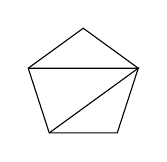
\begin{tikzpicture}[x=0.75pt,y=0.75pt,yscale=-0.5,xscale=0.5]
\draw (40.7,146.98) -- (93.72,108.46) -- (146.74,146.98) -- (126.49,209.31) -- (60.95,209.31) -- cycle ;
\draw (40.7,146.98) -- (146.74,146.98) -- (60.95,209.31);
\end{tikzpicture}
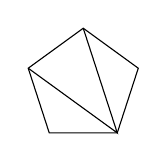
\begin{tikzpicture}[x=0.75pt,y=0.75pt,yscale=-0.5,xscale=0.5]
\draw (40.7,146.98) -- (93.72,108.46) -- (146.74,146.98) -- (126.49,209.31) -- (60.95,209.31) -- cycle ;
\draw (93.72,108.46) -- (126.49,209.31) -- (40.7,146.98);
\end{tikzpicture}
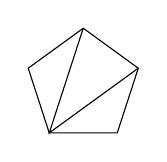
\begin{tikzpicture}[x=0.75pt,y=0.75pt,yscale=-0.5,xscale=0.5]
\draw (40.7,146.98) -- (93.72,108.46) -- (146.74,146.98) -- (126.49,209.31) -- (60.95,209.31) -- cycle ;
\draw (146.74,146.98) -- (60.95,209.31) -- (93.72,108.46);
\end{tikzpicture}
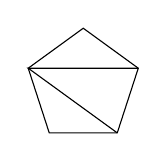
\begin{tikzpicture}[x=0.75pt,y=0.75pt,yscale=-0.5,xscale=0.5]
\draw (40.7,146.98) -- (93.72,108.46) -- (146.74,146.98) -- (126.49,209.31) -- (60.95,209.31) -- cycle ;
\draw (126.49,209.31) -- (40.7,146.98) -- (146.74,146.98);
\end{tikzpicture}
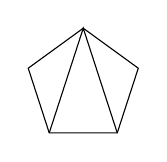
\begin{tikzpicture}[x=0.75pt,y=0.75pt,yscale=-0.5,xscale=0.5]
\draw (40.7,146.98) -- (93.72,108.46) -- (146.74,146.98) -- (126.49,209.31) -- (60.95,209.31) -- cycle ;
\draw (60.95,209.31) -- (93.72,108.46) -- (126.49,209.31);
\end{tikzpicture}
\caption*{5 Non-Overlapping Triangulations of a Pentagon}
\end{figure}

\begin{hl}
\begin{proof}
\;
\medskip

\begin{minipage}{0.69\linewidth}
Let $t_n$ count the number of triangulations of an $n$-gon. Pick an edge of the polygon. There are $n-2$ triangles it could belong to, since there are $n-2$ other vertices. In each case, it splits the polygon into two smaller ones with number of sides $k$ and $n+3-k$ for $2\leq k\leq n+1$. The number of ways to finish the triangulation is thus $t_{k-2}t_{n+1-k}$. Summing over all $k$, we have $\sum_{k=2}^{n+1}t_{k-2}t_{n+1-k}=\sum_{k=1}^{n}t_{k-1}t_{n-k}$. But this is the same recurrence as the Catalan Numbers in Theorem \ref{catalan_recur}. Since $t_2=1=c_0$ and $t_3=1=c_1$, we have that $t_{n+2}=c_n$.
\end{minipage}%
\begin{minipage}{0.3\linewidth}
\centering
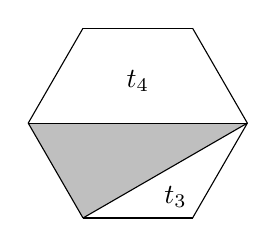
\begin{tikzpicture}[x=0.75pt,y=0.75pt,yscale=-0.4,xscale=0.4]
\path [fill=gray!50] (431.34,140.89) -- (233.39,255.18) -- (167.4,140.89) -- cycle;
\draw (431.34,140.89) -- (365.36,255.18);
\draw (365.36,255.18) -- (233.39,255.18);
\draw (233.39,255.18) -- (167.4,140.89);
\draw (167.4,140.89) -- (233.39,26.6);
\draw (233.39,26.6) -- (365.36,26.6);
\draw (365.36,26.6) -- (431.34,140.89);
\draw (431.34,140.89) -- (233.39,255.18);
\draw (431.34,140.89) -- (167.4,140.89);
\node at (299.375,90) {$t_4$};
\node at (345,230) {$t_3$};
\end{tikzpicture}
\end{minipage}

\medskip

Another proof bijects triangulations to full binary trees whose vertices are the $n+2$ exterior edges and the $n-1$ internal edges (resulting in $n+1$ leaf nodes). Fix an edge to be the root of the tree, and identify the triangle it belongs to. Let the other two edges be the children of the root. Now continue recursively. Any exterior edge encountered is a leaf node. For any internal edge, it borders two triangles: the one used to reach that edge, and a triangle not yet counted. Let the children of the edge be the other two edges of the uncounted triangle.

\medskip

A final proof bijects triangulations to parenthesizations. Label all except one of the edges, so that there are $n+1$ labeled edges. Now, iteratively label the interior edges by combining labels, using parentheses to specify the order in which they are combined. The final parenthesization is the label of the last exterior edge.

\begin{figure}[H]
\centering
\begin{subfigure}{0.6\linewidth}
\raisebox{-.5\height}{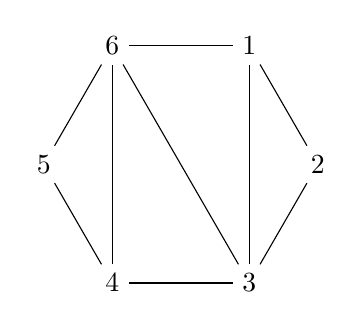
\begin{tikzpicture}[x=0.75pt,y=0.75pt,yscale=-0.5,xscale=0.5]
\node (1) at (431.34,140.89) {2};
\node (2) at (365.36,255.18) {3};
\node (3) at (233.39,255.18) {4};
\node (4) at (167.4,140.89) {5};
\node (5) at (233.39,26.6) {6};
\node (6) at (365.36,26.6) {1};
\path[-] (1) edge (2);
\path[-] (2) edge (3);
\path[-] (3) edge (4);
\path[-] (4) edge (5);
\path[-] (5) edge (6);
\path[-] (6) edge (1);
\path[-] (3) edge (5);
\path[-] (5) edge (2);
\path[-] (2) edge (6);
\end{tikzpicture}}
$\longleftrightarrow$
\raisebox{-.5\height}{\begin{forest}
[16
	[13
		[12]
		[23]
	]
	[36
		[34]
		[46
			[45]
			[46]
		]
	]
]
\end{forest}}
\caption*{Method 2}
\end{subfigure}%
\begin{subfigure}{0.3\linewidth}
\centering
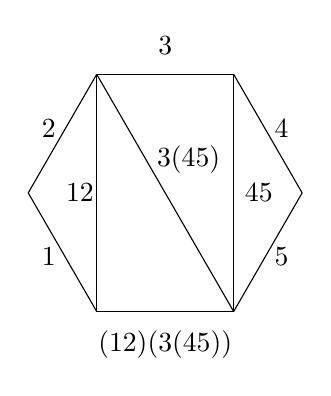
\begin{tikzpicture}[x=0.75pt,y=0.75pt,yscale=-0.5,xscale=0.5]
\draw   (431.34,140.89) -- (365.36,255.18) node [pos=0.3, label=below:{5}] {};
\draw (365.36,255.18) -- (233.39,255.18) node [pos=0.5, label=below:{(12)(3(45))}] {};
\draw (233.39,255.18) -- (167.4,140.89) node [pos=0.7, label=below:{1}] {};
\draw (167.4,140.89) -- (233.39,26.6) node [pos=0.3, label=2] {};
\draw (233.39,26.6) -- (365.36,26.6) node [pos=0.5, label=3] {};
\draw (365.36,26.6) -- (431.34,140.89) node [pos=0.7, label=4] {};
\draw (233.39,26.6) -- (365.36,255.18) node [pos=0.5, label=above right:{3(45)}, xshift=-1em] {};
\draw (233.39,26.6) -- (233.39,255.18) node [pos=0.5, label=left:{12}, xshift=0.6em] {};
\draw (365.36,26.6) -- (365.36,255.18) node [pos=0.5, label=right:{45}, xshift=-0.3em] {};
\end{tikzpicture}
\caption*{Method 3}
\end{subfigure}
\end{figure}
\end{proof}
\end{hl}
\end{theorem}

\begin{theorem}
Consider a string of parentheses that satisfies the criteria to be legal, except that not all left parentheses need to be closed. Let $q_n$ count the number of possible strings of length $n$. Then $q_n=\binom n{\lfloor n/2\rfloor}$, the Central Binomial Coefficients.

\begin{hl}
\begin{proof}
If no prefix exists, then removing the leading left parenthesis is a bijection to $q_{n-1}$. Otherwise, condition on the index, so that there are $\sum_{k=1}^{\lfloor n/2\rfloor}c_{k-1}q_{n-2k}$ options. Together, we have $q_n=q_{n-1}+\sum_{k=1}^{\lfloor n/2\rfloor}c_{k-1}q_{n-2k}$ for $n>0$ and $q_0=1$. The corresponding generating function is:
\begin{align*}
Q(x)
&=\sum_{n=0}^\infty q_nx^n
=q_0+\sum_{n=1}^\infty\left[q_{n-1}+\sum_{k=1}^{\lfloor n/2\rfloor}c_{k-1}q_{n-2k}\right]x^n
=1+\sum_{n=1}^\infty q_{n-1}x^n+\sum_{n=1}^\infty\sum_{k=1}^{\lfloor n/2\rfloor}c_{k-1}q_{n-2k}x^n\\
&=1+xQ(x)+\sum_{k=1}^{\infty}\sum_{n=2k}^\infty c_{k-1}q_{n-2k}x^n
=1+xQ(x)+\sum_{k=1}^{\infty}c_{k-1}x^{2k}\sum_{n=2k}^\infty q_{n-2k}x^{n-2k}\\
&=1+xQ(x)+Q(x)x^2\sum_{k=0}^{\infty}c_{k}x^{2k}
=1+xQ(x)+Q(x)x^2C(x^2)
\end{align*}

Solving:
\begin{align*}
Q(x)
&=-\frac{1}{x^2C(x^2)+x-1}
=-\frac{1}{\frac{1-\sqrt{1-4x^2}}{2}+x-1}
=\frac{2}{\sqrt{1-4x^2}-2x+1}\\
&=\frac{2(\sqrt{1-4x^2}+2x-1)}{(\sqrt{1-4x^2}-2x+1)(\sqrt{1-4x^2}+2x-1)}
=\frac{2\sqrt{1-4x^2}+4x-2}{1-4x^2-(2x-1)^2}
=\frac{2\sqrt{1-4x^2}+4x-2}{-8x^2+4x}\\
&=\frac{\sqrt{1-4x^2}+2x-1}{2x(1-2x)}
\end{align*}

Thus, using Theorem \ref{truncate_alt_binom}:
\begin{align*}
q_n
&=[x^n]Q(x)
=\frac12[x^n]\frac{\sqrt{1-4x^2}+2x-1}{x(1-2x)}
=\frac12[x^{n+1}]\left(\frac{\sqrt{1-4x^2}}{1-2x}-1\right)
=\frac12[x^{n+1}]\frac{\sqrt{1-4x^2}}{1-2x}\\
&=2^n[x^{n+1}]\frac{\sqrt{1-x^2}}{1-x}
=2^n\sum_{k=0}^{n+1}[x^k](1-x^2)^{1/2}
=2^n\sum_{k=0}^{n+1}[x^k]\sum_{k=0}^\infty\binom{1/2}k(-1)^kx^{2k}\\
&=2^n\sum_{k=0}^{n+1}[x^k]\sum_{k=0}^\infty[k\text{ even}]\binom{1/2}{k/2}(-1)^{k/2}x^{k}
=2^n\sum_{\substack{k=0\\k\text{ even}}}^{n+1}\binom{1/2}{k/2}(-1)^{k/2}\\
&=2^n\sum_{k=0}^{\lfloor\frac{n+1}2\rfloor}\binom{1/2}{k}(-1)^{k}
=2^n\binom{-1/2}{\lfloor(n+1)/2\rfloor}(-1)^{\lfloor(n+1)/2\rfloor}
=2^{n-2\lfloor\frac{n+1}2\rfloor}\binom{2\lfloor\frac{n+1}2\rfloor}{\lfloor\frac{n+1}2\rfloor}
\end{align*}

When $n$ is even, we obtain $\binom n{n/2}$. When $n$ is odd, we obtain $\frac12\binom{n+1}{(n+1)/2}=\frac12\frac{n+1}{(n+1)/2}\binom{n}{(n-1)/2}=\binom n{(n-1)/2}$. In either case, $q_n=\binom n{\lfloor n/2\rfloor}$.
\end{proof}
\end{hl}
\end{theorem}

\subsection{Counting Using Products}


\begin{example}
Suppose a semester of $n$ days is divided into two parts (of arbitrary length), and there is 1 holiday during the first part and 2 holidays during the second part. Let $s_n$ be the number of ways this can be accomplished. Condition on the number of days in the first part $k$. Choose the holiday in the first part $k$ ways, and choose the holidays in the second part $\binom{n-k}2$ ways. Thus, $s_n=\sum_{k=1}^{n-2}k\binom{n-k}2$.

\medskip

The appearance of this form suggests using the product of generating functions. Let $a_n=\binom n1$ and $b_n=\binom n2$, so that $S(x)=A(x)B(x)$. By Lemma \ref{binom_gen}:
\begin{equation*}
S(x)
=A(x)B(x)
=\frac{x}{(1-x)^2}\cdot \frac{x^2}{(1-x)^3}
=\frac{x^3}{(1-x)^5}
\end{equation*}

Thus, we compute:
\begin{equation*}
s_n
=[x^n]\frac{x^3}{(1-x)^5}
=[x^n]\frac1x\frac{x^4}{(1-x)^5}
=[x^{n+1}]\frac{x^4}{(1-x)^5}
=\binom{n+1}4
\end{equation*}
\end{example}

\section{Sieve Method}
\begin{theorem}[Principal of Inclusion/Exclusion]
Let $S$ be a collection of $N$ objects and let $P=\{p_1,\dots,p_r\}$ be a set of properties that one or more of the elements in $S$ possess. Let $N(p_{i_1},\dots,p_{i_n})$ count the number of objects that satisfy at least the properties $p_{i_1},\dots,p_{i_n}$, and let $P_i$ be the set of elements satisfying $p_i$. Let $e_j$ count the number of objects with exactly $j$ properties. Then:
\begin{equation*}
e_0
=\underbrace{N}_{N_0}-\underbrace{\sum_{j=1}^rN(p_j)}_{N_1}+\underbrace{\sum_{j<k}N(p_j,p_k)}_{N_2}-\underbrace{\sum_{j<k<\ell}N(p_j,p_k,p_\ell)}_{N_3}+\cdots+(-1)^r\underbrace{N(p_1,\dots,p_r)}_{N_r}
\end{equation*}

Alternatively, the number of objects satisfying at least one property is:
\begin{equation*}
\left|\bigcup_{j=1}^rP_j\right|
=N_1-N_2+\cdots+(-1)^{r+1}N_r
\end{equation*}

The number satisfying at least $j$ properties is similarly computed, and by taking differences, the number satisfying exactly $j$ properties can be computed. Or, using generating functions $E(x)=\sum_ke_kx^k$ and $N(x)=\sum_kN_kx^k$, we have $E(x)=N(x-1)$, so that expanding $N(x-1)$ gives us all values of $e_j$.
\begin{hl}
\begin{proof}
We have $N_k=\sum_{j=k}^r\binom jke_j$ by conditioning on the number of properties $j$ and then picking $k$ to use. Then the generating functions satisfy:
\begin{equation*}
N(x)
=\sum_{k=0}^rN_kx^k
=\sum_{k=0}^r\sum_{j=k}^r\binom jke_jx^k
=\sum_{j=0}^re_j\sum_{k=0}^j\binom jkx^k
=\sum_je_j(1+x)^j
=E(1+x)
\end{equation*}

Then $E(x)=N(x-1)$. Substituting $x=0$ yields $e_0=N(-1)=\sum_kN_k(-1)^k$.
\end{proof}
\end{hl}
\end{theorem}

\begin{example}
Consider counting the derangements in $S_n$, as in Example \ref{derangements}. Letting $N=n!$ and $p_j$ be the property that the permutation fixes $j$, then $N(p_j)=(n-1)!$, $N(p_j,p_k)=(n-2)!$, and so on. Thus:
\begin{align*}
!n
&=n!-\sum_{j}(n-1)!+\sum_{j<k}(n-2)!-\sum_{j<k<\ell}(n-3)!+\cdots+(-1)^r(n-n)!\\
&=n!-\binom n1(n-1)!+\binom n2(n-2)!-\binom n3\sum_{j<k<\ell}(n-3)!+\cdots+(-1)^r\binom nn(n-n)!\\
&=\sum_{j=0}^n\binom nj(n-j)!(-1)^j
=n!\sum_{j=0}^n\frac{(-1)^j}{j!}
\end{align*}
\end{example}

\begin{example}
The number of nonnegative integer solutions to $x_1+x_2+x_3=17$ is given by the number of weak compositions as $\multbinom 3{17}=\binom{19}2=171$. If we add the restriction that $x_1\leq 6$, $x_2\leq10$, and $x_3\leq8$, then this can be counted using Inclusion/Exclusion with properties $p_1=(x_1>6)$, $p_2=(x_2>10)$, and $p_3=(x>8)$. Allocating the 7 guaranteed parts to $x_1$, we obtain that $N(p_1)=\multbinom 3{17-7}=\multbinom3{10}=66$, and similarly $N(p_2)=\multbinom3{6}=28$, $N(p_3)=\multbinom 38=45$, $N(p_1p_2)=0$, $N(p_1p_3)=\multbinom 31=3$, $N(p_2p_3)=0$, and $N(p_1p_2p_3)=0$. Then the total number of given by $171-66-28-45+3=35$.
\end{example}
\end{document}
